%%%%%%%%%%%%%%%%%%%%%%%%%%%%%%%%%%%%%%%%%%%%%%%%%%%%%%%%%%%%%%%%%%%%%%%%
\chapter{Modellbasiertes Testen in agilen Entwicklungsumgebungen}
\chaptermark{Modellbasiertes Testen}
\label{sec:problemdescription}
%%%%%%%%%%%%%%%%%%%%%%%%%%%%%%%%%%%%%%%%%%%%%%%%%%%%%%%%%%%%%%%%%%%%%%%%

Dieses Kapitel enthält eine Beschreibung der im Zuge dieser Arbeit durchgeführten Fallstudie beim Partnerunternehmen Raiffeisen Schweiz Genossenschaft. Die Struktur des Softwareprojekts, in dem der Autor die in Kapitel \ref{sec:results} \Newnameref{sec:results} vorgestellte modellbasierte Teststrategie erproben konnte, wird in Abschnitt \ref{sec:fallstudie} erklärt. In den darauffolgenden Abschnitten werden verschiedene Ansätze und Werkzeuge für modellbasiertes Testen auf mehreren Testebenen beschrieben und auf Eignung für den Einsatz in agilen Projekten bewertet.

\section{Fallstudie: Kundenberaterapplikation einer Schweizer Bank}
\sectionmark{Fallstudie}
\label{sec:fallstudie}
\subsection{Hintergrund zu den Applikation RETo und RESi}
Die Applikation \textit{RESi}, in anderer Struktur und bis in das Jahr 2013 \textit{RETo} (Raiffeisen Expert Tool), ist ein \Gls{Back-End}-Service, das Dienste für die verschiedensten \Gls{Front-End}-Applikationen des Unternehmens bereitstellt. \textit{RESi} bietet sozusagen eine \Gls{SOA}. Unter altem Namen bot die Applikation früher eine eigene Benutzeroberfläche und weniger, dafür spezifischere, Funktionalität. RETo war im Intranet der Filialen im Einsatz und wurde ausschließlich für Kundenberatungen eingesetzt. Die Applikation hatte folgende Kernkompetenzen:

\begin{itemize}
\item Ermittlung von Anlegerprofilen
\item Durchführung von Anlage-Checks
\item Beratungen zum Thema Wohnen und Wohneigentum
\item Beratungen zum Thema Vorsorge
\item Beratungen zum Thema Pension
\end{itemize}

Im Jahr 2014 wurde ein Großteil der Applikationslandschaft umstrukturiert. In einer Bemühung, einzelne Applikationen zu vereinheitlichen und Mehrfachaufwendungen zu minimieren, wurde RETo modularisiert. Das Projekt RESi wurde gestartet. RESi stellt eine Back-End-Service Schicht dar. Da RETo bereits einen sehr breiten Funktionsumfang bot, besteht RESi zu großen Teilen aus den RETo Kernkomponenten. Auch das Entwicklungsteam ist dasselbe geblieben. Mehrere, ehemals eigenständige Applikationen, greifen jetzt auf RESi zu und bieten nur noch ein Front-End und eine dünne Serverschicht. RETo existiert weiterhin, aber greift auch auf die Services von RESi zu.

\subsection{Entwicklungsumfeld}
Das Umfeld der Applikation RESi wird in einem Auftragnehmer/Auftraggeber-Szenario entwickelt. Eine Fachabteilung stellt den Kunden dar. Sie definiert die Anforderungen an die Applikation. Demgegenüber steht das Entwicklungsteam, welches aus einem Applikationsmanager und 8-10 Entwicklern besteht. Die Entwicklung findet unter folgenden Gesichtspunkten statt:

\begin{itemize}
\item 2 Major Releases pro Jahr
\item Mehrere Service-Releases pro Jahr
\item Dreiwöchige Scrum-Sprints
\item 4 Ebenen (Integrationstest, Systemtest, Akzeptanztest, Produktion)
\item Scrum Master wechselt
\item Product Owner (PO) wird von Fachbereich gestellt
\item tägliche Scrum-Meetings
\end{itemize} 

Die Applikation RESi ist, bedingt durch ihre Reife, bereits sehr stabil. Effektiv ist sie schon seit ungefähr 8 Jahren (in anderer Struktur und unter anderem Namen) im produktiven Einsatz. Der typische Entwicklungszyklus wird vom Fachbereich angestoßen. Ein \gls{RFC} wird vom Fachbereich angenommen oder verfasst. Die zuständigen Produktmanager definieren genügend fachliche Details, bevor ein \gls{RFC} in eine \gls{Story} verwandelt wird (siehe Abschnitt \ref{sec:scrum} für eine Einführung in agile Methoden). Diese \gls{Story} fließt nun typischerweise in den \gls{Backlog}. Wenn auf einer der Entwicklungsebenen Fehler mit hoher Priorität gefunden werden, wird eine Beschreibung des Fehlverhaltens verfasst, die direkt in die laufende Entwicklungsiteration einfließt.\\
Auf Seiten der Entwickler finden kurze tägliche Meetings statt. Dauer und Struktur dieser täglichen Meetings entsprechen den klassischen Daily-Scrum-Standup-Meetings. Neben den Entwicklern ist der Scrum-Master und der Product Owner aus dem Fachbereich anwesend. Er steht für kurzfristig auftretende Fragen bereit. Weiters finden im Entwicklungsteam wöchentliche Research-Meetings statt. In diesen werden die neu eingetroffenen Storys analysiert und modularisiert. Ziel ist es, eine Story in kleinere Tasks herunterzubrechen, die in einem Arbeitstag schaffbar sind. Ein Task soll also von einem einzelnen Entwickler implementiert werden. Im selben Zug werden die Aufwände der Story und damit der Tasks geschätzt. Im RESi-Team kommt folgende Methode zur Aufwandsschätzung zum Einsatz. Einerseits wird eine Methode verwendet, in der alle Storys offen und ungeordnet aufgelegt werden. Nun wird das Team der Reihe nach gebeten, eine Story einzuordnen. Damit werden weder Storypoints noch Stunden geschätzt. Storys werden anhand ihrer augenscheinlichen Aufwände geordnet. Wenn kein Teammitglied mehr eine Änderung machen will, endet die Aufwandsschätzung. Der Scrum-Master legt schlussendlich, in Absprache mit dem Team, fest, welcher Bereich von Storys in einen zukünftigen Sprint fließt. Storys aus dem vorderen Bereich der Reihung sind dementsprechend die zeitintensivsten. So können Storys ausgewählt werden um die verfügbare Zeit in einer Entwicklungsiteration möglichst gut auszufüllen.

\subsection{Entwicklungsebenen}
Zwischen der Implementierung einer Funktion und deren Eintritt in eine produktive Umgebung läuft diese durch definierte Ebenen. Während der Implementierung einer Funktion benutzen die Entwickler eine lokale Installation der Applikation (diese entspricht der Ebene \textit{Integrationstest}). Wenn ein Entwickler die Programmierung der Funktion abschließt und alle Komponententests erwartungsgemäß durchlaufen werden, wird diese zum \gls{Review} freigegeben. Ein anderer Entwickler liest den Code und gibt Feedback zu Richtigkeit, Effizienz, Lesbarkeit und Stil. Der Code wird, nach eventueller Korrektur, auf der Ebene \textit{Integrationstest} deployed (ein IBM WebSphere Applikationsserver \footnote{IBM WebSphere \url{http://www.ibm.com/websphere}} im Falle von RESi). Diese Ebene hat die Hauptaufgabe, auftretende Nebeneffekte aufzudecken, die der neu implementierte Code verursacht. Ab diesem Zeitpunkt beginnt der Fachbereich bereits mit manuellen Tests auf der Integrationsumgebung. In manchen Fällen macht es keinen Sinn, gegen einzelne Funktionen zu testen (möglicherweise lassen sich diese GUI-seitig auch gar nicht testen). Dann wird abgewartet, bis verwandte Funktionen oder die ganze zugehörige Story für den Integrationstest freigegeben werden. Da Entwickler und Fachbereich täglich auf dieser Ebene arbeiten, werden auftretende Nebeneffekte durch Wartungsänderungen eher entdeckt.\\
Nach Abschluss eines Sprints wird der Stand der Ebene \textit{Integrationstest} auf \textit{Systemtest} deployed. Hier testet der Fachbereich genau definierte Abläufe manuell. Außerdem unternimmt auf dieser Ebene eine gesonderte Testabteilung Last- und Performancetests. Bis zu diesem Zeitpunkt läuft die Entwicklung streng nach agilen Prinzipien. Um das Zusammenspiel der Applikationslandschaft zu vereinheitlichen, wird unternehmensweit aber immer noch auf viel längere Release-Zyklen gesetzt. Sprint-Ergebnisse werden nicht zeitnah in die Produktionsebene versetzt. Die Ebene \textit{Akzeptanztest} wird zwischen Systemtest und \textit{Produktionsebene} gezogen. Auf ihr werden die Stände getestet, die für Major-Releases geplant sind. Typischerweise wird gegen Ende eines Major-Release Zyklus verstärkt auf der Ebene \textit{Akzeptanztest} deployed und getestet. Trotzdem kann es zu Überlappungen kommen, die mit dem agilen Iterationszyklus interferieren. Sprint-Ergebnisse die kurz vor einem Major-Release eigentlich für die Produktionsreife getestet werden sollten, werden möglicherweise erst für die nächste Veröffentlichung beachtet. Erstens werden also Testressourcen periodisch für \textit{Akzeptanztest} benötigt, obwohl bereits neuere Versionen der Applikation testbar wären. Zweitens leidet das Endprodukt, wenn Features, die eigentlich zur Veröffentlichung freigegeben werden könnten, mehrmonatige Verspätungen haben.

\subsection{Qualitätssicherung im Projekt}
\label{sec:quality_project}
In die Entwicklung und Qualitätssicherung des Produkts sind diverse Parteien involviert. Anfänglich, also zum Zeitpunkt der Anforderungsanalyse und der Spezifikationsentwicklung, sind auch Teams involviert, die während der Entwicklung und Wartung nicht mehr beteiligt sind. Dazu zählen auch externe Mitarbeiter.\\
Während der Wartungsphase des Systems gibt es einen Testverantwortlichen. Diese Rolle befindet sich auf Seiten der nicht-technischen Produktmanager. Der Testverantwortliche delegiert und orchestriert die Erstellung und Durchführung von manuellen Testfällen. Alle Teams benutzen zum Requirement- und Testmanagement HP QualityCenter \footnote{HP QualityCenter Internetauftritt \url{http://www8.hp.com/us/en/software-solutions/quality-center-quality-management/}}. Dies hat den Vorteil, dass übergreifend alle Beteiligten über den Status des Produkts genau informiert sind. Manuelle Testfälle und Testfallsuiten sind meist textuell beschrieben und manchmal als \gls{COS}-Tabellen definiert. Diese \gls{COS}-Tabellen haben eine hohe Ähnlichkeit zu Skripts, die beim Einsatz von automatisierten GUI-Tests zum Einsatz kommen (siehe Abbildung \ref{fig:cos_raiffeisen}). Angegeben werden ``Vorher''- und ``Nachher''-Zustände sowie die auszuführenden Aktionen. Der Detailgrad kann erheblich variieren.

\begin{figure}[h] 
  \centering
     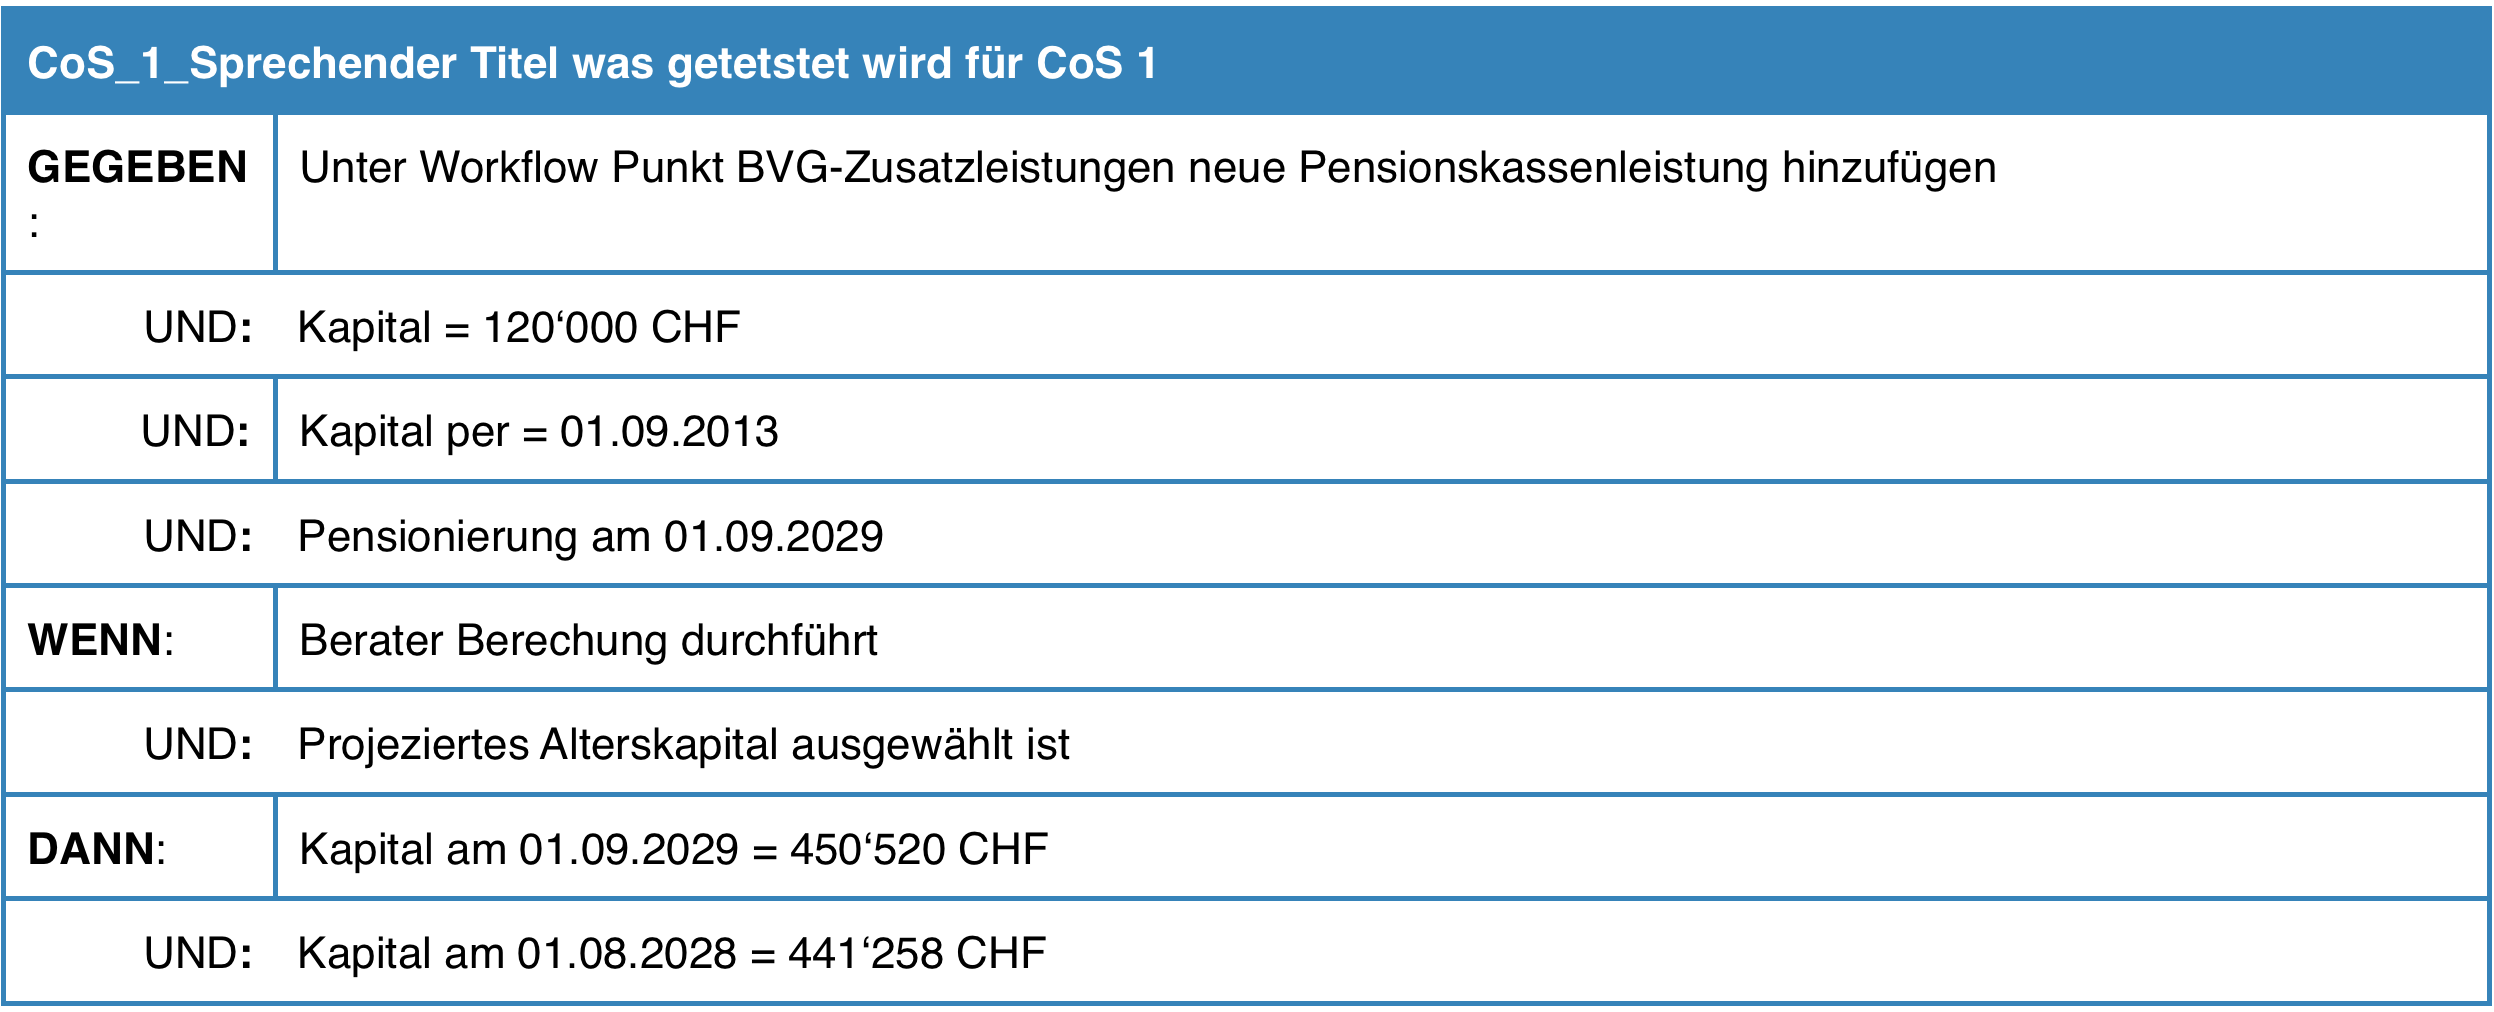
\includegraphics[width=0.9\textwidth]{figures/cos_raiffeisen.png}
  \caption{Muster-COS-Tabelle wie sie von den Testfalldesignern verwendet werden.}
  \label{fig:cos_raiffeisen}
\end{figure}


Auf Seiten der Entwickler, also im Scrum-Team, gibt es keinen dedizierten Tester. Im Entwicklungszyklus sind nur Unit-Tests fixiert. Weiters werden vom Testverantwortlichen auch den Entwicklern manuelle Testfälle zugewiesen, die im Rahmen des Integrationstests durchgeführt werden.

\subsubsection{Erkannte Schwachstellen in der Qualitätssicherung}
\label{sec:schwachstellen_raiffeisen}
Für diese Fallstudie wurden Interviews mit dem leitenden Architekten der Applikation, einem Entwickler, einer Business-Analystin und einem Testverantwortlichen geführt. Der dabei verwendete Leitfaden findet sich im Anhangskapitel \ref{app:leitfaden}. Die hier dargestellten Punkte stellen eine Zusammenfassung aller gesammelten Meinungen dar.\\
\begin{itemize}
\item \textbf{Zuständigkeitsbereiche sind nicht klar kommuniziert:} An den Softwareprojekten sind verschiedenste Teams beteiligt. Dazu zählen die langzeitigen Projektmitglieder aus dem Entwicklungsteam, Business-Analysten und Fachbereich aber auch punktuell beteiligte Teams. Außerdem gibt es Teams die als Dienstleister am Projekt beteiligt sind und beispielsweise Lasttests durchführen. Zwischen den Teams gibt es definierte Kommunikationspunkte. Beispielsweise stellt das Team der Business-Analysten den Product-Owner. Dieser fungiert als Schnittstelle und synchronisiert Anliegen beider Parteien. Aufgrund der großen Anzahl an Beteiligten fehlt der Gesamtüberblick über die Zuständigkeitsbereiche und Tätigkeitsfelder der einzelnen Personen und Teams. Nicht alle Prozesse der miteinander arbeitenden Teams sind dem Gegenüber bekannt. Dies ist meist auch nicht nötig, aber in manchen Fällen hilft es, die eigenen Anstrengungen besser aufeinander abzustimmen.
\item \textbf{Unsaubere Trennung der Verantwortlichkeiten:} Die vielen beteiligten Parteien haben allesamt einen Aufgabenbereich. Über die Länge des Projekts gesehen gibt es aber offene Punkte, die nicht klar einem Zuständigkeitsbereich zugeordnet sind. Zum Beispiel werden von Business-Analysten manuelle Regressionstests ausgeführt und die Fachbereiche führen in niedrigerer Frequenz manuelle Abnahmetests durch. All diese Anstrengungen sind aber nicht mit der Qualitätssicherung koordiniert, die von den Entwicklern vorgenommen wird.
\item \textbf{Spezifikationen haben keine einheitliche Form:} Die Definition von User-Storys und den dazugehörigen \Gls{COS} geschieht nach keinem durchgängigen Muster. Auch die Anzahl und das Design der \Gls{COS} selbst ist innerhalb des Projekts unterschiedlich. Das fachliche Testfalldesign ist nicht transparent. Unsystematische Tests können zulassen, dass gravierende Fehler im \Gls{SUT} nicht aufgedeckt werden.
\end{itemize}

\subsubsection{Verbesserungspotenzial}
\label{sec:massnahmen}
Die oben erwähnten Schwächen könnten, auf Grund der gesammelten Erfahrung des Autors und der Vorschläge der interviewten Personen, folgendermaßen verbessert werden:

\begin{itemize}
\item \textbf{Mehr Kommunikation über Teamgrenzen hinweg:} Während der Fallstudie wäre es von Vorteil gewesen früher zu wissen, dass der Fachbereich zwingend \Gls{COS}-Tabellen für ihre Abnahmetests vorschreibt. In welcher Form Abnahmetests im Detail gemacht werden, ist auf Seiten der Entwickler nicht ganz klar. Es handelt sich hierbei also um Kommunikationshürden, die die Gesamtheit des Projekts betreffen und durch optimierten Informationsfluss beseitigt werden müssen.
\item \textbf{Einbeziehen des Fachbereichs:} Hier bestünde großes Potenzial das Testen effizienter zu machen, wenn das Team der Business-Analysten stärker in die Erstellung und Wartung automatisierter Regressionstests miteinbezogen werden könnten.
\item \textbf{Form der Spezifikationen klar definieren:} Unter Einbezug aller beteiligten Teams sollte klar gemacht werden, wie aus Spezifikationen die dazugehörigen \Gls{COS} definiert werden. Zuvor muss sich das spezifizierende Team auf eine einheitliche Form einigen.
\end{itemize}


\subsubsection{Versuch der Qualitätssicherung durch skriptgesteuerte GUI-Tests}
\label{sec:versuch_script}
Vor wenigen Jahren wurde im Projektteam versucht die manuellen Aufwände für das Regressionstesten auf GUI-Ebene zu minimieren. Nach sorgfältiger Evaluation der sich auf dem Markt befindlichen Werkzeuge wurden skriptgesteuerte Tests eingesetzt, die einen Benutzer simulieren. Auf diesem Weg erhoffte man sich manuelle \Gls{COS}-Tests teilweise zu ersetzen. Nach wenigen Monaten stellte sich aber heraus, dass der Wartungsaufwand für die sich schnell entwickelnden Systeme schlichtweg zu hoch war. Außerdem war der Qualitätsgewinn durch die nächtlich laufenden Testfälle gering, weil sich das Werkzeug nur unzureichend in den Entwicklungsprozess integrieren ließ und die Rate der falschen Positivfälle sehr hoch war.\\
Wartungsaufwände, die beim skriptbasierten Testen anfielen, konnten ausschließlich von technischem Personal durchgeführt werden. Eine sinnvolle Aufteilung der erhöhten Belastung durch das Testen war so nicht möglich.

\subsubsection{Aufwendige Wartung von Testdaten}
In der Domäne der Finanzapplikationen ist es üblich, dass eine Vielzahl von Datenfeldern spezifiziert werden. Wie für die Branche üblich, handelt es sich dabei oft um numerische Werte. Um bei solchen Systemen eine zufriedenstellende Abdeckung zu erreichen, ist es nötig, mit hoher Kombinatorik zu testen. Dies setzt den Einsatz von umfangreichen Testdatensätzen voraus. Auch die Ablaufverfolgung von Testdaten (welcher Bereich der Testdaten wird von einem bestimmten Testfall benutzt) und Testfällen ist ein Thema. Beim Design einer sinnvollen Teststrategie muss darauf geachtet werden, dass eine Entkopplung von Verhalten und Daten gemacht wird. Wenn Daten eng an das Verhalten im Testfall gebunden sind, führt dies zu einem stark erhöhten Wartungsaufwand \cite{baker_model-driven_2005}. 

%%%%%%%%%%%%%%%%%%%%%%%%%%
\section{Kein Modellformat hat sich als Standard etabliert}
\label{sec:discussion_format}
%%%%%%%%%%%%%%%%%%%%%%%%%%%
Die Auswahl des Modellformats und die zugrunde liegende Notation ist eine fundamentale Entscheidung bei der Einführung von modellbasiertem Testen. Meist geht die Auswahl eines \Gls{MBT} Werkzeugs mit der Wahl des Modellformats einher. Die Ursprünge dieser Werkzeuge, für welche Art von Softwareprojekten diese zumeist eingesetzt wurden, sind unschwer an der unterstützten Modellnotation zu erkennen.  In der Praxis besteht eine Vielzahl von Notationen und Formaten, die auf sehr unterschiedlichen Prinzipien beruhen. Eine Transformation von einem Modellformat in ein anderes ist kaum möglich (beispielsweise lässt sich ein Modell in B Notation nur mit genauer Kenntnis des \Gls{SUT} in die Graphwalker-Notation konvertieren.)\\
Erschwerend kommt hinzu, dass gerade die großen kommerziellen Werkzeuge (wie Leiros Smartesting \footnote{Leiros Smartesting Produktseite \url{http://www.smartesting.com/en/}} oder Conformiq's \Gls{MBT} Toolsuite \footnote{Conformiq Produktseite \url{https://www.conformiq.com/products/}}) vollständig auf nicht-portable Eigenentwicklungen setzen. Diese Hersteller versuchen gezielt große Software-Projekte in ihr Ökosystem einzusperren, verpassen es aber die Branche der \Gls{MBT} Werkzeuge voranzutreiben. Sie vermarkten ihre Modellformate als Produktgeheimnis und verhindern dadurch die Entwicklung eines Standards, der modellbasiertes Testen viel stärker in Erscheinung treten ließe. Weiters lassen sich Fähigkeiten der Werkzeuge kaum vergleichen. Während die Firma Conformiq ohne weiteres Testversionen ihrer vollständigen Toolsuite anbietet und die Open-Source Werkzeuge ohnehin frei evaluierbar sind, verlangt die Firma Leiros knapp 1000 Euro für eine akademische Lizenz. Auch auf Nachfrage des Autors wurde keine Demo- oder Testversion zum Zweck dieser Diplomarbeit zur Verfügung gestellt. Anhand offizieller Produktbeschreibungen und Quellen lässt sich nicht herausfinden, wie sich der Workflow mit dem genannten Programm verhält, geschweige denn, wie die zugrunde liegende Modellierung funktioniert.\\
Die Bemühungen der \Gls{OMG} mit dem \Gls{UTP} eine einheitliche Sprache für modellbasiertes Testen zu schaffen ist ebenfalls nicht gelungen. Die Zahl der Publikationen die sich auf das UML Testing Profile stützen ist seit 2007 zwar konstant \footnote{Nach Recherche auf einschlägigen Portalen wie \url{http://ieeexplore.ieee.org/}}, trotzdem bietet kein dem Autor bekanntes Werkzeug Unterstützung dafür an. Zwar schlägt die offizielle Publikation der \Gls{OMG} \cite{_model-driven_2007} manuelle Vorgehensweisen zur Benutzung von \Gls{UTP} vor (siehe Kapitel \ref{sec:utp}), dies ist im Umfeld großer agiler Softwareprojekte aber nicht praktikabel. Zu viele Fehler könnten bei der manuellen Transformation von \Gls{UTP}-Diagramme passieren.\\
Im Kontext von skriptbasierten GUI-Tests hat sich gezeigt, dass eine Herstellerunabhängigkeit mittel- bis langfristig von Vorteil ist. Diese Fallstudie war ebenfalls in der Finanzbranche angesiedelt \cite{graham_experiences_2012}. Die Fallstudie dieser Arbeit (siehe Abschnitt \ref{sec:fallstudie} \Newnameref{sec:fallstudie}) hat gezeigt, dass diese Erkenntnis auch im Umfeld des modellbasierten Testens gilt. Die Verwendung eines nicht-proprietären Modellformats bringt, abgesehen von der Flexibilität und Ungebundenheit, mehrere Vorteile:

\begin{itemize}
\item \textbf{Portabilität und Lesbarkeit:} Sollte ein Wechsel der Entwicklungsplattformen oder sogar der Teststrategie bevorstehen, können Modelle, die in einem offenen Format wie XML serialisiert werden, mühelos transformiert werden. Es bleibt aber zu beachten, dass Transformationen zwischen fundamental verschiedenen Modellierparadigmen, trotz offener Serialisierung, kaum machbar sind.
\item \textbf{Wiederverwendbarkeit:} Leichtgewichtige und quelloffene Werkzeuge, wie Graphwalker, erlauben die Weiterbenutzung bestehender skriptbasierter Tests. In der Praxis hat sich außerdem gezeigt, dass es sehr vorteilhaft ist, Teile der Testbasis iterativ auf modellbasierte Tests zu übertragen. Der Aufbau der Modellierungskenntnisse im Team geschieht so breitflächiger und leichtgängiger, als wenn eine große Menge von Modellen und Adaptercode auf einmal erstellt werden müssen. Aus Sicht des Managements müssen weniger Aufwände initial riskiert werden, um projektrelevante Erfahrungen mit \Gls{MBT} zu sammeln. Aus Sicht der Entwickler besteht viel Freiraum in der Werkzeugauswahl für Adaptercode.
\item \textbf{Transparenz:} Technisch versierte Tester bzw. Testentwickler schätzen es, wenn das Parsen des Modells und die Testfallgenerierung möglichst transparent passieren. Bei omnipotenten \Gls{MBT} Lösungen ist dies nicht der Fall, da sie diese Details vor dem Benutzer verbergen wollen um attraktiv für die Fachbereiche zu wirken. In der Praxis sind aber Entwickler sowohl in der Auswahl des Werkzeugs als auch in der Erstellung der Modelle stark beteiligt.
\end{itemize}

%%%%%%%%%%%%%%%%%%%%%%%%%%%%%%%%%%%%%%%%%%%%%%%%%%%%%%%%%%%%%%%%%%%%%%%%
\section{MBT auf Komponententestebene anhand von ModelJUnit}
%%\label{sec:mbt_unit}
%%%%%%%%%%%%%%%%%%%%%%%%%%%%%%%%%%%%%%%%%%%%%%%%%%%%%%%%%%%%%%%%%%%%%%%%
\label{sec:modeljunit}
ModelJUnit wird von Dr. Mark Utting et al. an der Universität Waikato in Neuseeland entwickelt. Es wird unter der Open-Source-GNU-GPL-Lizenz entwickelt und befindet sich zur Zeit in der Version 2.5 \footnote{Homepage des Tools ModelJUnit \url{http://www.cs.waikato.ac.nz/~marku/mbt/modeljunit/}}. Es erlaubt die Modellierung des \Gls{SUT} als endlichen Automaten (siehe Abschnitt \ref{sec:fsm} für eine Einführung in endliche Maschinen) in Java, Generierung von Testfällen laut spezifiziertem Traversierungsalgorithmus sowie das Erstellen von Auswertungen. Seit Version 2.0 bietet das Werkzeug eine grafische Benutzeroberfläche, die die Traversierungskonfiguration ermöglicht und veranschaulicht.\\
ModelJUnit hat Ähnlichkeiten zu Graphwalker (siehe Abschnitt \ref{sec:graphwalker}), indem es eine Schicht zur Modellierung anbietet und die Traversierung des \gls{SUT} übernimmt, aber keine Aussage darüber trifft, wie das \gls{SUT} angesprochen werden soll. Der Adapter-Code wird also in annotierte Methoden eingefügt. ModelJUnit übernimmt die Traversierung. Das Modell, welches keine grafische Notation bietet, besteht aus Zuständen und Übergängen, dies entspricht einem gerichteten Graphen. Die Zustände und Knoten haben Bezeichner, außerdem können auf den Kanten sogenannte \textit{Guards} definiert werden. Dies sind WahrFalsch-Methoden, die bestimmen ob zu einem gegebenen Zeitpunkt diese Kante zur Traversierung verfügbar ist oder nicht. Der Testentwickler hat fast unbegrenzte Möglichkeiten, Guard-Bedingungen zu überprüfen, da es sich um Java-Code handelt.

\subsection{Modellierung der States}
Jedes Modell wird als Java-Klasse definiert. Eine gültige ModelJUnit-Modellklasse implementiert mindestens die folgenden vier Zustände. 

\begin{itemize}
\item \texttt{Object getState()} Diese Methode gibt den momentanen Zustand des SUT, so wie er im Modell repräsentiert wird, zurück. Im einfachsten Fall ist dies eine Abstraktion als String, es können aber beliebige Objekte zurückgegeben werden.
\item \texttt{void reset(boolean)} Setzt die Traversierung und die Zustände des Modells auf den Startzustand zurück.
\item \texttt{@Action void name()} Mehrere Methoden werden mit dieser Annotation gekennzeichnet. Sie stellen die Zustandsübergänge dar. In ihnen wird das \Gls{SUT} angesprochen.
\item \texttt{boolean nameGuard()} Jede Methode, die mit \texttt{@Action} annotiert ist, kann optional einen Guard haben. Per Definition muss diese Methode denselben Namen wie die dazugehörige Action haben, aber mit dem Postfix \texttt{Guard} versehen sein.
\end{itemize}

Die Zustände, in denen sich das \Gls{SUT} während einem ModelJUnit Test befindet, werden als Enum definiert. Im Konstruktor der Klasse wird der Startzustand des Modells gesetzt. In jeder \texttt{Action}-Methode wird typischerweise ein kurzer Aufruf an das \Gls{SUT} gemacht. Die Aneinanderkettung dieser kurzen Komponententestähnlichen Aufrufe während der Traversierung resultiert in komplexen Testfällen.\\
Abbildung \ref{fig:modeljunit} zeigt wie ein in Java-Code geschriebenes Modell grafisch visualisiert werden könnte.  ModelJUnit selbst besitzt keinerlei grafische Notation und erzeugt auch kein grafisches Modell. Diese Nachbildung dient nur der besseren Vorstellung.

\begin{figure}[h] 
  \centering
     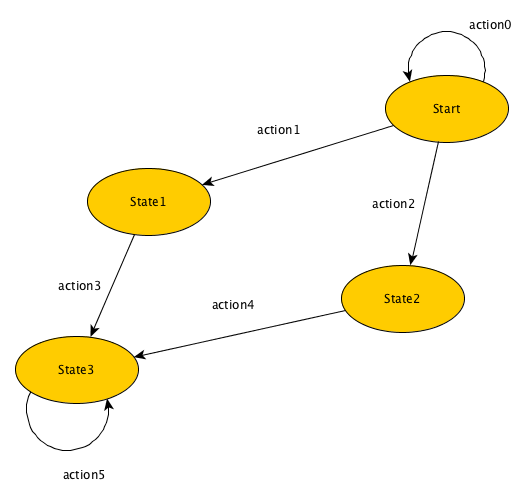
\includegraphics[width=0.9\textwidth]{figures/modelljunit_modell.png}
  \caption{Ein beispielhaftes syntaktisch korrektes Modell, wie es von ModelJUnit eingelesen wird.}
  \label{fig:modeljunit}
\end{figure}

\subsection{Traversierung}
Die Definition einzelner Testfälle, also die Aneinanderreihung von Schritten, durch den Testentwickler entfällt. Nach der Modellierung muss nur die gewünschte Traversierungsstrategie gewählt werden. ModelJUnit bietet einige der bekanntesten Traversierungsalgorithmen. Für alle Traversierungsalgorithmen gelten die Grenzen, die durch Guards aufgestellt werden.

\paragraph{Random Walk}
Das Modell wird zufällig traversiert, bis ein Zielknoten erreicht wurde oder eine zeitliche Grenze überschritten wurde.

\paragraph{Greedy Walk}
Die Greedy-Walk-Strategie ist eine Erweiterung des Random Walks. Sie bevorzugt Zustandsübergänge, die noch nicht traversiert wurden. Sobald alle Zustandsübergänge mindestens einmal traversiert wurden, verhält sich Greedy Walk wie Random Walk.

\paragraph{Lookahead Walk}
Der Lookahead-Walk-Algorithmus schaut vor jedem Schritt $n$ Ebenen voraus. Drei Kriterien werden dabei ausgewertet: \textit{NEWTRANS}, \textit{NEWACTION} und \textit{DEPTH}. Das Erreichen eines noch unbekannten Zustandes hat die höchste Priorität, wobei ein kurzer Pfad vorzuziehen ist. Außerdem verlieren öfter traversierte Pfade an Attraktivität: Dies bewirkt, dass in möglichst kurzer Zeit jeder Pfad mindestens einmal traversiert wird.

\paragraph{Quick Walk}
Traversiert den Graphen ähnlich wie Random Walk, speichert aber in einem Cache die entdeckten, aber noch nicht traversierten Pfade. Außerdem speichert der Algorithmus den exakten Pfad zu jedem nicht besuchten Knoten und dessen Pfade. Ein Cache-Limit muss angegeben werden, um bei sehr großen Modellen vor Überlauf geschützt zu sein.

\subsection{Einsatz von ModelJUnit}
ModelJUnit nutzt die Ausdrucksstärke und Flexibilität von Java. Es können alle Kerneigenschaften der Sprache für die Modellierung verwendet werden. Java ist vielen Entwicklern bereits bekannt. Die Entscheidung, ModelJUnit zu verwenden, zieht somit keine langwierigen Schulungen nach sich. Außerdem integriert sich ModelJUnit sehr einfach in bestehende Strukturen, wie zum Beispiel die Continiuous-Integration-Umgebung.\\
Im Gegensatz zu sehr formalen Modellierungssprachen verbergen sich Guard- und Übergangsbedingungen innerhalb von Methoden. Sie werden nicht in ausdrucksstarken kurzen Annotationen festgehalten. Weiters kann sich viel Komplexität in diesen Methoden verstecken und vom Umstand ablenken, dass das \Gls{SUT} falsch oder zu abstrakt modelliert wurde. Diese Eigenschaft haben alle \Gls{MBT} Werkzeuge, die Modelle aus der Familie der endlichen Automaten verwenden.

%%%%%%%%%%%%%%%%%%%%%%%%%%%%%%%%%%%%%%%%%%%%%%%%%%%%%%%%%%%%%%%%%%%%
\section{MBT auf Integrationstestebene}
\label{sec:mbt_integration}
%%%%%%%%%%%%%%%%%%%%%%%%%%%%%%%%%%%%%%%%%%%%%%%%%%%%%%%%%%%%%%%%%%%%

\subsection{Testen von serviceorientierten Architekturen mittels UML Testing Profile}
\label{sec:utp}
\glsreset{SOA}
Am Beispiel von \glspl{SOA} soll der folgende Abschnitt erläutern, wie modellbasiertes Testen mittels dem UML Testing Profile für das Testen auf Integrationsebene eingesetzt werden kann. 

\subsubsection{Das UML Testing Profile}
Die \Gls{UML} wird in der Softwareentwicklung seit langer Zeit gelehrt und verwendet. Es handelt sich dabei um eine grafische Modellierungssprache zur Spezifikation, Konstruktion und Dokumentation von Softwaresystemen. \Gls{UML} Profile können als Spezialisierung von \Gls{UML} gesehen werden \cite{_model-driven_2007}. Ein Profil kann die ursprüngliche Sprache an gewissen Stellen erweitern, aber auch einschränken. Ein Beispiel ist das \Gls{UTP}. Dieses Profil führt Konzepte ein, die es ermöglichen, Testspezifikationen und Testmodelle als bekannte \Gls{UML}-Modelle darzustellen. Die Autoren \cite{_model-driven_2007} haben versucht, die Mehrheit der Konzepte und Visualisierungen für \Gls{UTP} an die Version 2 von \Gls{UML} anzulehnen. Benutzern, denen die Grundsprache \Gls{UML} bekannt ist, sollte es nicht schwer fallen mit \gls{UTP} umzugehen.\\
Im Folgenden werden die von \Gls{UTP} neu eingeführten Begrifflichkeiten beschrieben. Nicht alle haben eine grafische Repräsentation:

\begin{itemize}
\item \textbf{Testarchitektur} Die Testarchitektur ist die Menge der Modelle und Komponenten um die strukturellen Aspekte einer Testsituation in ihrer Gesamtheit darzustellen. Dabei wird auf das Vokabular von \Gls{UML} 2.0 und \Gls{UTP} zurückgegriffen.
\item \textbf{Testkontext} Der Testkontext ordnet und gruppiert die Menge der einzelnen Tests und lässt Schlüsse auf die Ausführungsdetails zu.
\item \textbf{Testkonfiguration} Die Testkonfiguration stellt dar, wie Kommunikation zwischen den weiteren Testkomponenten und dem \Gls{SUT} verläuft. Das \Gls{SUT} kann aus einer oder mehreren Komponenten bestehen. Abbildung \ref{fig:utp_config} zeigt eine Testkonfiguration, die aus einem zweiteiligen \Gls{SUT} besteht, zwei Testkomponenten (\texttt{tb:TBorrower} und \texttt{tl:TLibrarian}) sowie einem \textit{Data Pool} (siehe Abschnitt \ref{sec:utp_datapools} für eine Beschreibung dieses wichtigen \Gls{UTP} Konzepts).
\item \textbf{Testkomponenten} Die Testkomponenten sind beliebige Objekte innerhalb des Testsystems, die mit anderen Komponenten oder dem \Gls{SUT} kommunizieren und eine gewisse Funktionalität mit sich bringen.
\end{itemize}

Die von \Gls{UTP} eingeführten Komponenten werden stets in Stereotyp-Notation im grafischen Modell gekennzeichnet (siehe Abbildung \ref{fig:utp_config} bei \texttt{<<TestComponent>>}).

\begin{figure}[h] 
  \centering
     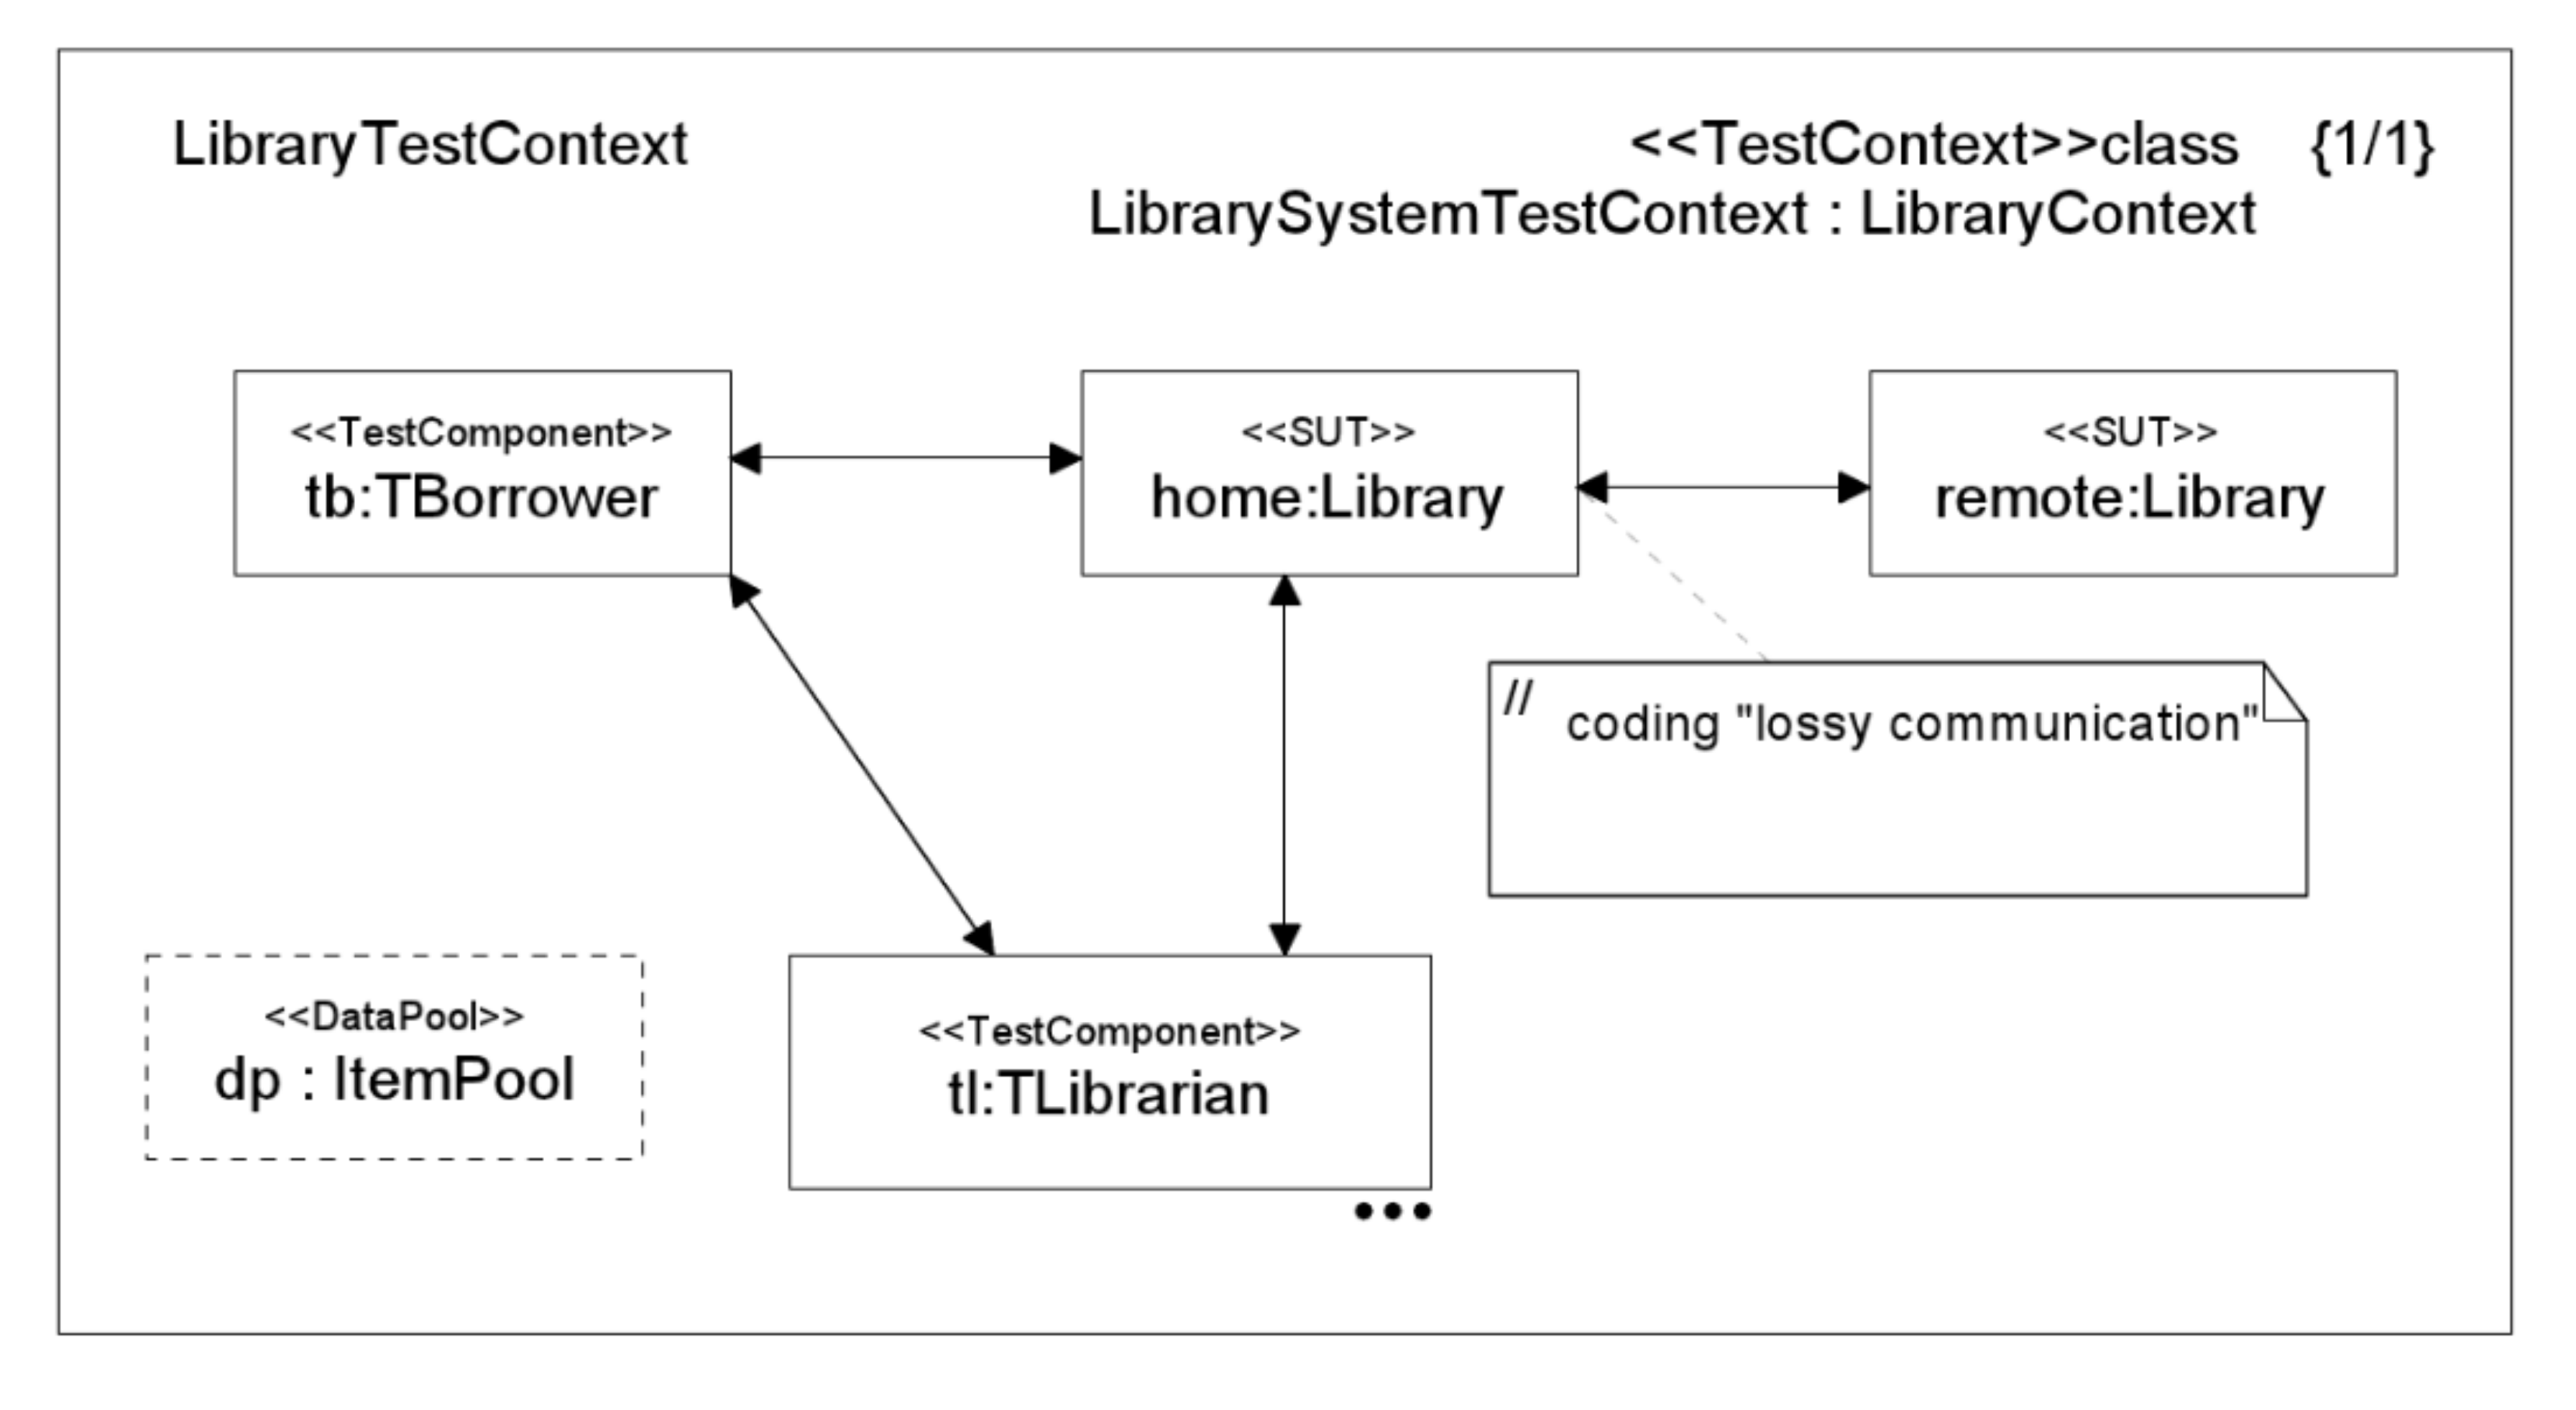
\includegraphics[width=0.9\textwidth]{figures/utp_config.png}
  \caption{Eine beispielhafte UTP Testkonfiguration aus \citetitle{_model-driven_2007} \cite{_model-driven_2007}}
  \label{fig:utp_config}
\end{figure}

Zur Darstellung der Testfälle wird auf bekannte \Gls{UML} Komponenten zurückgegriffen. Denkbar sind Zustandsdiagramme, Aktivitätsdiagramme oder, wie im Beispiel \ref{fig:utp_case}, Interaktionsdiagramme. In diesem Testfall werden die aus der Testkonfiguration (Abbildung \ref{fig:utp_config}) bekannten Akteure in einen Ablauf gebracht. Zu sehen sind die Testkomponenten \texttt{TBorrower} und \texttt{TLibrarian}, die Aktionen auf dem \Gls{SUT} ausführen. Ein Konzept, welches nicht innerhalb des \Gls{UML} 2.0 Standards definiert wird, sind die Zeitmesser (\textit{Timer}). In diesem Fall sollen sie Zeitschranken zwischen der Anfrage der Testkomponente und der Antwort des \Gls{SUT} darstellen.

\begin{figure}[h] 
  \centering
     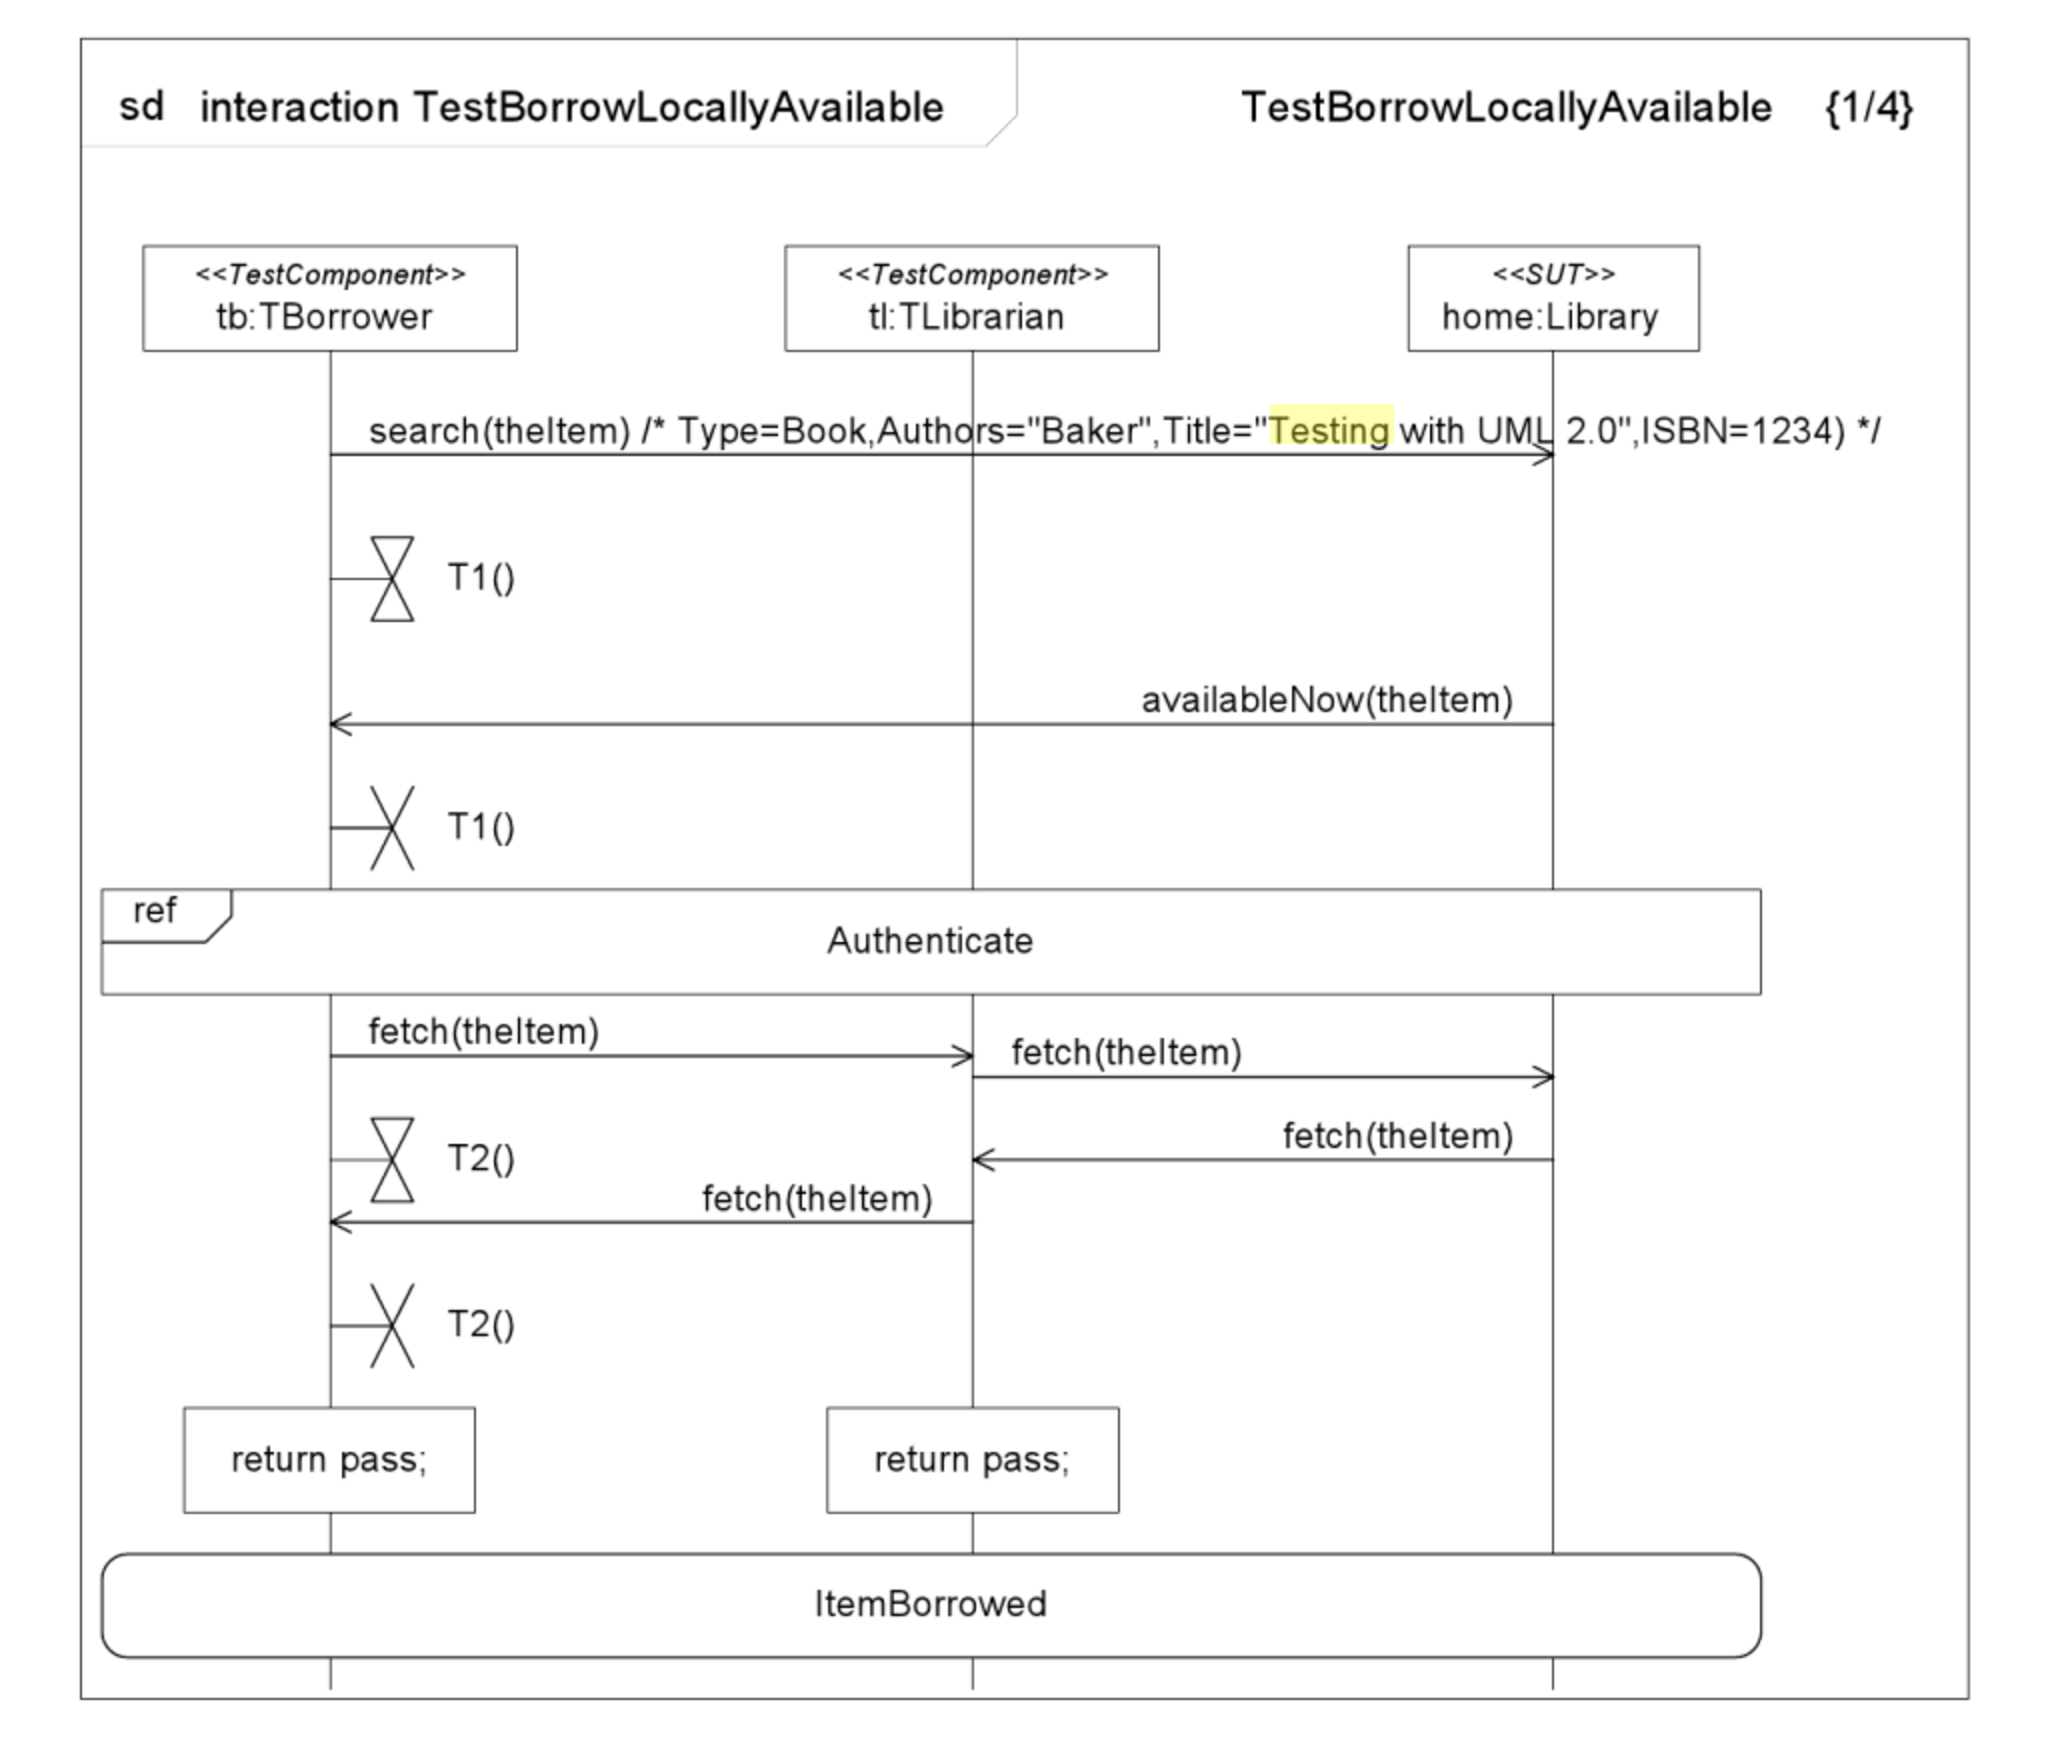
\includegraphics[width=0.9\textwidth]{figures/utp_case.png}
  \caption{Ein UTP Testfalldiagramm aus \citetitle{_model-driven_2007} \cite{_model-driven_2007}}
  \label{fig:utp_case}
\end{figure}

\subsubsection{Testdatenkonzept in UTP}
\label{sec:utp_datapools}
Das allgemeinste Konzept für den Umgang mit Daten in \Gls{UTP} sind Platzhalter (\textit{Wildcards}). Diese können überall dort eingesetzt werden wo unerwartete Werte vorkommen dürfen. Ein Platzhalter sagt aus, dass jeder beliebige Wert valide ist.\\
Für Fälle, in denen genaue Testdaten eingesetzt werden müssen, bietet \Gls{UTP} \glspl{datapool} und, hierarchisch darunter, \glspl{datapartition}. Erstere stellen eine Entität innerhalb des \Gls{SUT} dar, die in gewisse Äquivalenzklassen, die \glspl{datapartition}, unterteilt werden. \glspl{datapool} werden stets in einer Testkonfiguration eingesetzt (zu sehen in Abbildung \ref{fig:utp_config}). Abbildung \ref{fig:utp_pool} veranschaulicht, weiterhin am Bibliotheksbeispiel, einen \Gls{datapool}, der drei assoziierte \glspl{datapartition} besitzt.

\begin{figure}[h] 
  \centering
     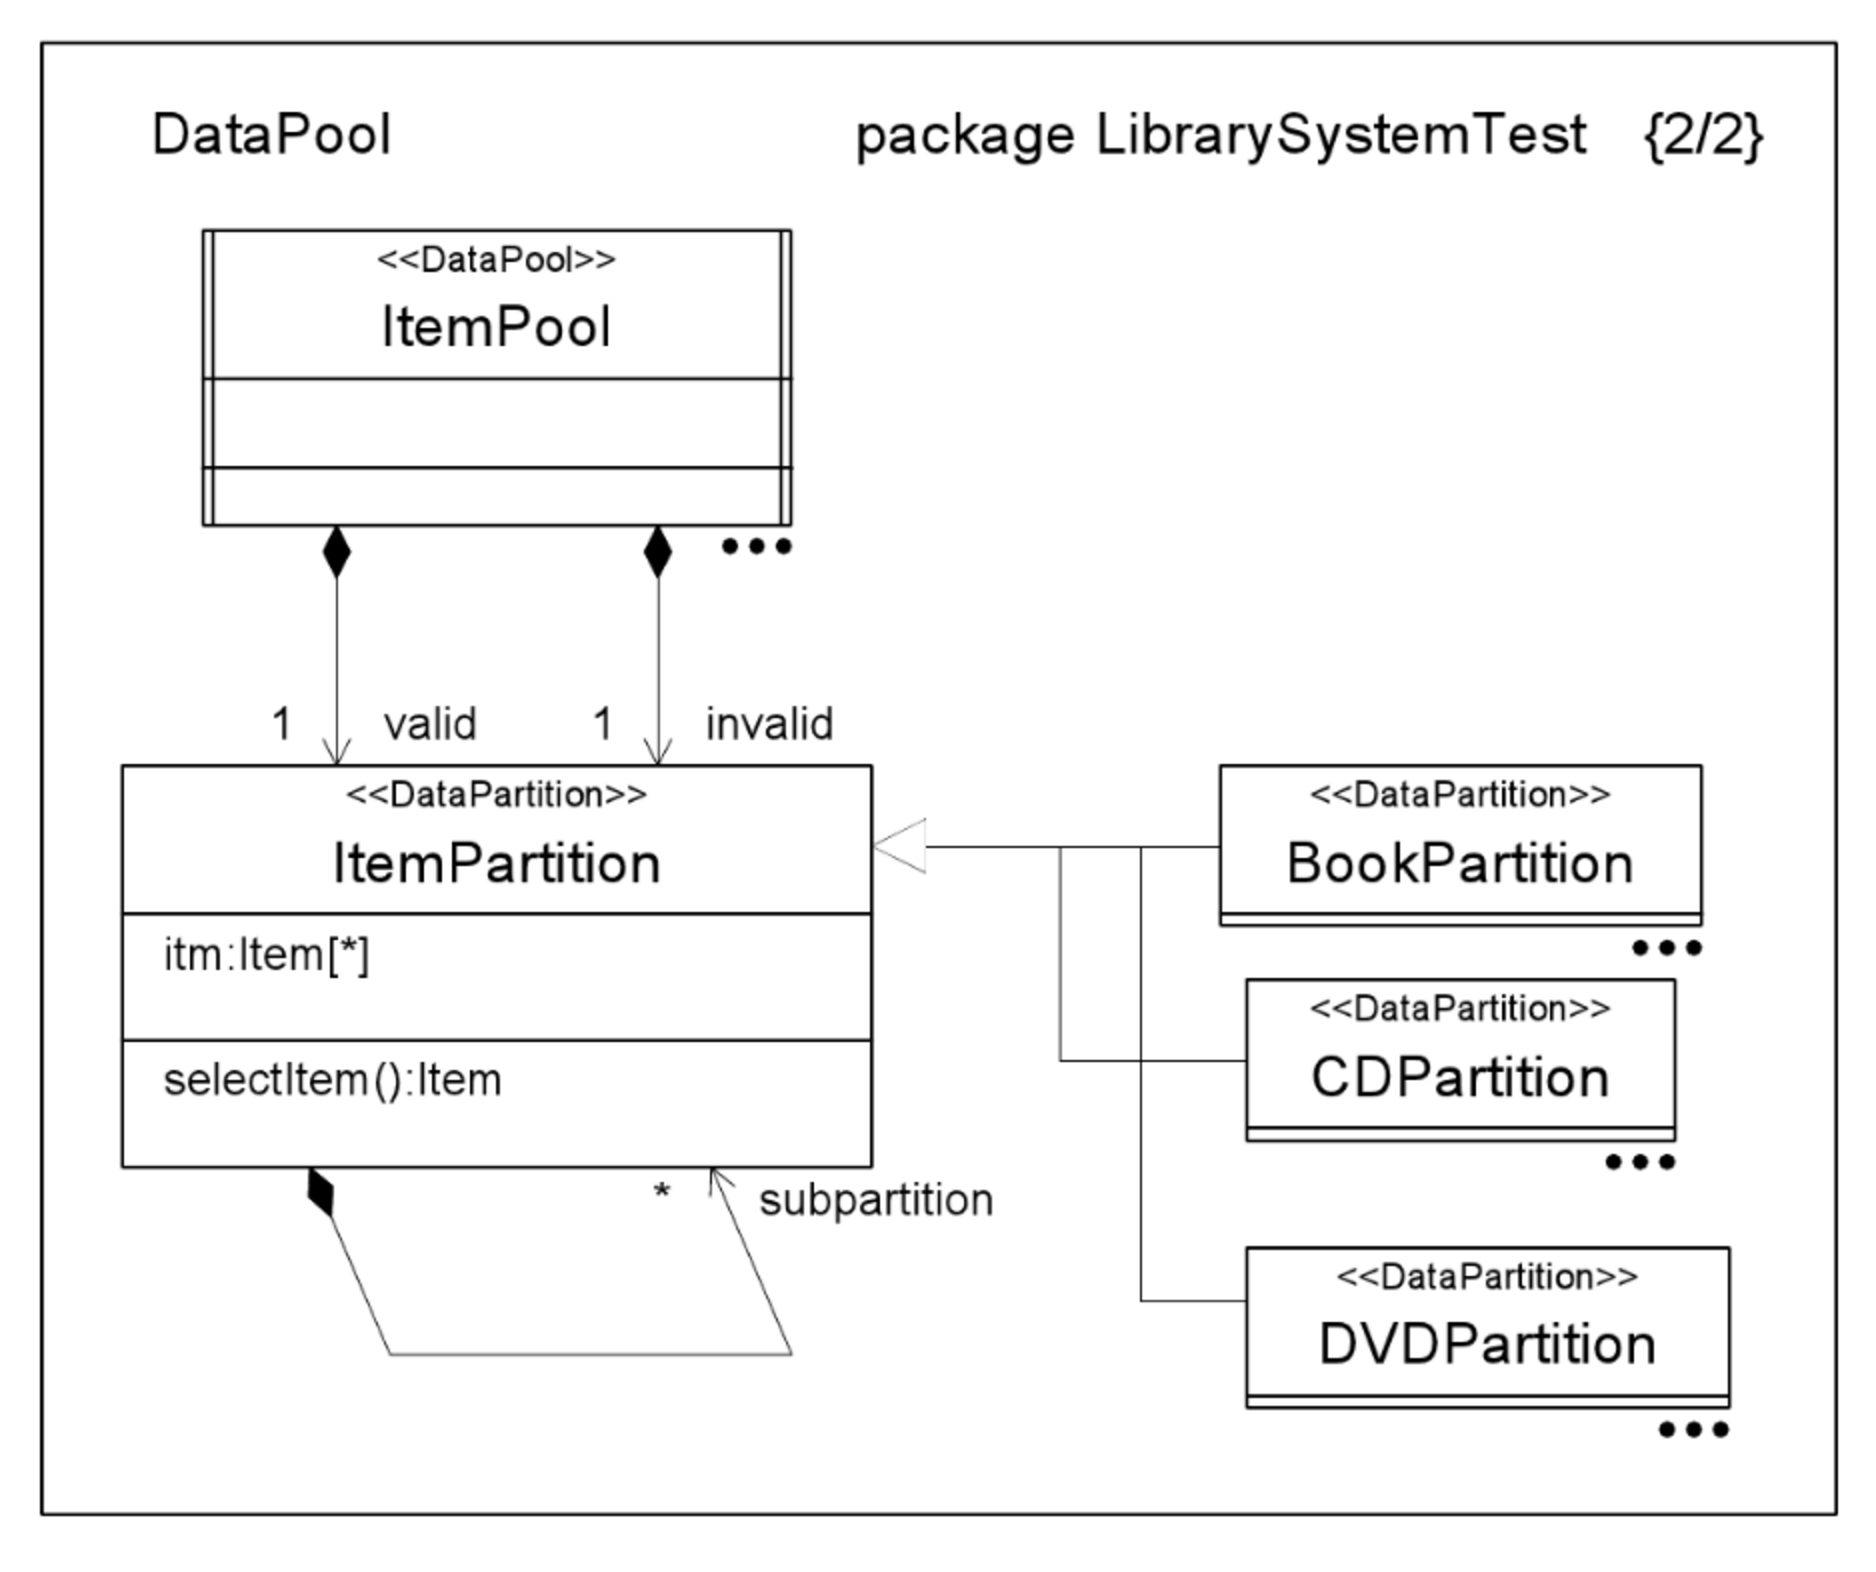
\includegraphics[width=0.9\textwidth]{figures/utp_pool.png}
  \caption{Umgang mit Testdaten in UTP: Data Pools und Data Partitions. Beispiel aus \citetitle{_model-driven_2007} \cite{_model-driven_2007}}
  \label{fig:utp_pool}
\end{figure}

\Gls{UTP} definiert noch weitere Konzepte und Komponenten. Diese sind für die Ergebnisse dieser Arbeit aber nicht relevant.

\subsubsection{Serviceorientierte Architekturen und Web-Services}
Von \glspl{SOA} verspricht man sich schnelle und einfache Integration, sowohl innerhalb des Unternehmens als auch über Unternehmensgrenzen hinweg. Die Möglichkeit, eine Applikation mittels Komposition, maßgeschneidert zu den gegebenen Anforderungen, zusammenzustellen, ist traditionellen Softwareentwicklungsmethoden oft voraus. Gleichzeitig stellen verschachtelte und unabhängige Strukturen den Tester vor neue Herausforderungen. \\
SOA wird missbräuchlich oft mit Web-Services gleichgestellt. Tatsächlich sind Web-Services nur die häufigste architektonische Grundlage für Applikationen mit  serviceorientierter Architektur. Die folgende Sektion geht ebenfalls von einer Serviceorientierten Architektur basierend auf Web-Services aus.

\subsubsection{Mapping von Web-Service Elementen auf UML-Diagramme}
Am Beispiel eines Web-Services, der per WSDL\footnote{WSDL Web-Service Spezifikationssprache 2.0 \url{http://www.w3.org/TR/wsdl20/}} definiert ist, soll gezeigt werden, wie eine Modellierung von Web-Services mittels dem UML-Testing Profile umgesetzt werden kann\footnote{Sehr ähnlich würde eine Modellierung für RESTful Web-Services basierend auf WADL ausschauen. Hierbei stellt sich aber eine Grundsatzfrage: Eines der Prinzipien von REST ist die Fähigkeit, dass sich ein Web-Service selbst beschreiben kann. Inwiefern trotzdem WADL Dateien gebraucht werden, hängt von der jeweiligen Implementierung ab.}. \citeauthor{_model-driven_2007} schlagen folgende Vorgehensweise für das Mapping vor \cite{_model-driven_2007}:

\begin{itemize}
\item WSDL \textit{Port Types} werden zu \Gls{UML} Stereotyp-Klassen gemappt.
\item Die Operationen in dieser Klasse stellen die Operationen dar, die der jeweilige Port Type offenbart.
\item Jede Operation hat eine übereinstimmende \textit{Request Message}. Falls die Operation auch einen Rückgabewert definiert, wird auch dieser abgebildet.
\item Komplexe Typen als auch Enumerationen werden zu stereotypisierten Klassen.
\end{itemize}

\subsubsection{Teststrategie für Web-Services}
Im Gegensatz zu herkömmlichen Desktop-Applikationen aus einer Hand können SOA Web-Services tief verschachtelte Komponenten von verschiedensten Parteien enthalten. Dies erschwert das Testen auf zwei Arten. Erstens können gravierende Qualitätsunterschiede zwischen Web-Services bestehen. Zweitens unterliegen diese Web-Services eigenen Wartungs- und Änderungsintervallen. Diese Erkenntnisse haben zur Folge, dass an die Teststrategie für Web-Services folgende zusätzliche Anforderungen gestellt werden:

\begin{itemize}
\item Tests müssen schnell und oft durchführbar sein (nämlich dann wenn eine Komponente geändert wird): \textit{On-Demand Testing}.
\item Gleichzeitig müssen die Tests kompakt und schnell wartbar sein (ähnlich Komponententests).
\item Web-Services sollen einzeln getestet werden können. Dies ermöglicht nicht nur eine gewisse Modularität, die zu einer hohen Testgeschwindigkeit beiträgt, sondern erleichtert auch die Fehlersuche bei einem negativen Testdurchlauf.
\end{itemize}

Web-Services müssen \textit{mehrdimensional} getestet werden \cite{_model-driven_2007}. Das bedeutet, ein modellbasierter Testfall soll alle Port Types, die der Service zur Verfügung stellt, kombiniert mit allen Operationen, die jeder Port Type anbietet, prüfen. Die Äquivalenzklassen aller Datentypen, die der Service bietet, müssen als Testdaten identifiziert werden. 
%Als Testdaten müssen die Äquivalenzklassen aller Datentypen, die der Web-Service anbietet, identifiziert werden.

\subsubsection{Beispielhafte Testsuite eines SOA Web-Services}
In diesem Beispiel wird ein Service einer Bücherei oder einer Buchhandlung herangezogen. Einfachheitshalber bietet dieser Service nur einen Port Type (\texttt{LibraryService}) an. Auf diesem werden drei Operationen angeboten (\texttt{search, reserve, fetch}). Die Abbildungen \ref{fig:utp_config} und \ref{fig:utp_case} stellen das Testsystem dar. Ein Client kann ein Element aus dieser Bücherei also suchen und basierend auf seinem Status-Parameter handeln. Das Element kann sofort verfügbar, später verfügbar und nicht lokal verfügbar sein.\\

Um die angesprochene mehrdimensionale Abdeckung zu gewährleisten bietet \Gls{UTP} das Konzept der Data Pools (siehe Abschnitt \ref{sec:utp_datapools}). Der DataPool stellt das kartesische Produkt dar, das aus Operationen und Datenelementen gebildet wird. Nun kann ein Testtreiber auf diesem Data Pool operieren und auf Testfalldiagramme (UML-Sequenzdiagramme) referenzieren.\\
Anhand von diesem einfachen Beispiel wird sichtbar, dass das \Gls{UML} Testing Profile sinnvolle Erweiterungen definiert, die die Modellierung von modernen SOA-Applikationen vereinfachen. Data Pools visualisieren die Abdeckung von Äquivalenzklassen und modularisierte Sequenzdiagramme erlauben die Modellierung von umfangreichen Testfällen. 

\subsubsection{Ausführung von UTP Tests mittels JUnit}
Agile Praktiken haben die Wahrnehmung der Wichtigkeit des Komponententests erhöht \cite{_model-driven_2007}. Ansätze wie \gls{Test-First} sind in diesem Umfeld besonders populär und der klassische Komponententest spielt dabei eine zentrale Rolle. Die Grundlagen des Komponententests wurden im Abschnitt \ref{sec:unit_test} erläutert.\\

Zum Zeitpunkt dieser Arbeit gibt es kein Werkzeug, welches die automatische Generierung von JUnit-Testfällen aus \Gls{UTP}-Modellen erlaubt. Das bedeutet, um \Gls{MBT} basierend auf \Gls{UTP}-Modellen in einem realen Umfeld zu betreiben, muss das Mapping manuell gemacht werden. \citeauthor{_model-driven_2007} schlagen dabei die in Tabelle \ref{table:utp_mapping} beschriebene Vorgehensweise vor \cite{_model-driven_2007}:

\begin{table}[h]
\centering
\begin{tabular}
{ | l |p{9cm}|} \hline
\textbf{UML Testing Profile} & \textbf{JUnit} \\ \hline \Gls{SUT}                       & Kein direktes Mapping nötig. Jede Klasse im \textit{Classpath} kann angesprochen und getestet werden   \\ \hline
Context                   & Kein direktes Mapping. JUnit kann auf den realen Kontext des \Gls{SUT} zugreifen. Aufwände außerhalb der JUnit-Programmierung sind nötig um alternative Konfigurationen zu testen \\ \hline
Runner         			  & JUnit bietet die Klasse \textit{org.junit.runner.Runner} um feingradige Einstellungen am Testablauf zu machen. \\ \hline
Scheduler   & Alle vom Java-Umfeld bereitgestellten Möglichkeiten der Scheduler sind einsetzbar (auch \textit{org.junit.runner.Runner} bietet Scheduler-Optionen) \\ \hline
Test configuration        & Implizit gegeben in JUnit, durch die direkte Einbindung der Klassen die getestet werden. \\ \hline
Test objective            & Dieses Konzept bietet JUnit nicht. Methoden können höchstens mit entsprechenden Kommentaren versehen werden.\\ \hline
Test case                 & Eine Methode die mit der Annotation \textit{@Test} versehen ist. \\ \hline
Test invocation           & Aufrufe der Methoden die mit \textit{@Test} annotiert sind. Üblicherweise durch einen Test-Runner. \\ \hline
Arbiter                   & Die Klassen \textit{org.junit.runner.Runner} und \textit{org.junit.runner.notification.RunListener} entscheiden über die Bewertung des Ausgangs eines Testfalls. Diese Klassen können bei Bedarf auch erweitert werden. \\ \hline
Verdict                   & Vordefinierte Testfallergebnisse sind \textit{pass}, \textit{fail} und \textit{error}. Auch diese Klasse kann um mehr Funktionalität erweitert werden. \\ \hline
Defaults                  & JUnit bietet keinen vergleichbaren Mechanismus.  \\ \hline
Validation action         & Validation Actions mappen auf die vielfältigen Methoden der Klasse \textit{org.junit.Assert} \\ \hline
Stimulus and observation  & Keine entsprechende Funktionalität in JUnit. \\ \hline
Logging concepts          & Im Java-Umfeld gibt es verschiedenste Logging-Frameworks die mit JUnit verwendet werden können. \\ \hline
Test data management: Data pools & Es sind keine entsprechenden Konzepte in JUnit vorhanden. \\ \hline
Test data managements: Wildcards  & Es sind keine entsprechenden Konzepte in JUnit vorhanden.\\ \hline
Timer                     & Es sind keine entsprechenden Konzepte in JUnit vorhanden. \\ \hline
Timezone                  & Es sind keine entsprechenden Konzepte in JUnit vorhanden. \\ \hline
Deployment       & JUnit fügt sich im Deployment Prozess sehr gut ein. \\ \hline
\end{tabular}
\caption{Mapping von UML Testing Profile zu JUnit}
\label{table:utp_mapping}
\end{table}

\Gls{UTP} wurde entwickelt, um mit JUnit zusammenzuspielen \cite{_model-driven_2007}. Tatsächlich lassen sich viele Konzepte gut von \Gls{UTP}-Modellen nach JUnit übertragen. Gleichzeitig hat die Ausführung von \Gls{UTP}-Testfällen in JUnit gravierende Schwächen:

\paragraph{Manuelles Mapping} Es hat sich in den Jahren, seit das \Gls{UML} Test Profile veröffentlicht wurde, keine Community um die Nutzung und Entwicklung von Software gebildet, die \Gls{UTP} einschließt. Die Eigenentwicklung eines JUnit-Testfallgenerators kann im Umfeld von großen Softwareprojekten sinnvoll sein. Gleichzeitig bleibt der Aufwand, um den sogenannten \textit{Adapter Code} zu schreiben (also die Implementierungsdetails innerhalb der Testmethoden).\\
Jedenfalls können durch einen manuellen Eingriff neue Fehler entstehen. Ein Modell mittels Testfällen umzusetzen ist kein trivialer Vorgang und erfordert genaue Kenntnisse des Frameworks sowie des \Gls{SUT}. Ob sich die Modellierung und die Aufwände für die Umsetzung in JUnit-Testfällen lohnen, lässt sich im Rahmen dieser Arbeit nicht feststellen. Faktisch bietet die Modellierung als \Gls{UTP} Diagramm zwar strukturierte Testfälle (verglichen mit der Ad-Hoc Entwicklung von JUnit-Testfällen), aber keine weiteren Qualitätsmetriken. Entwicklungsumgebungen und statische Code-Analyse-Werkzeuge können die Abdeckung von JUnit-Testfällen eruieren, diese sollte in agilen Softwareprojekten aber ohnehin schon sehr hoch sein. Ein modellbasierter Ansatz mit massiven manuellen Eingriffen kann hier wenig belegbare Qualitätsvorteile schaffen.

\paragraph{Keine Unterstützung der Testdatenmangementkonzepte}
Vor allem das \textit{Data Pool} Konzept von \Gls{UTP} ist eine Notwendigkeit für datenintensive Applikationen. Datengetriebene Testfälle müssen durch ein flexibles und zuverlässiges Konzept gestützt werden. Auch hier müsste eine Eigenentwicklung erstellt werden. Diese ist aber nicht nur aufwendig, sondern es stellt sich auch die Frage der Zukunftssicherheit. Kann das Modul zum Testdatenmanagement mit anderen Technologien verwendet werden oder ist es zu stark auf \Gls{UTP} zugeschnitten?

\subsection{Schnittstellentests mit Graphwalker}
\label{sec:graphwalker}
Graphwalker\footnote{Graphwalker-3-Website inklusive Dokumentation \url{www.graphwalker.org}} ist ein Open-Source-\Gls{MBT} Werkzeug zur Online- und Offline-Generierung von Testsequenzen aus Endlichen Automaten (siehe Abschnitt \ref{sec:fsm}) sowie Erweiterten Endlichen Automaten (EFSM). Graphwalker ist in Java und JavaScript implementiert und bietet eine Java-API an. Das Graphwalker-Projekt wurde von zwei Entwicklern der Firma Spotify\footnote{Der Musik-Streaming-Service Spotify \url{www.spotify.com}}, Nils Olsson und Kristian Karl, gegründet. Bei Spotify, dem marktführenden Musik-Streaming-Service, ist das Werkzeug auch stark im Einsatz. Graphwalker ist zur Zeit (Frühjahr/Sommer 2015) aktiv unter Entwicklung und liegt bereits in der Version 3.0 vor.\\
Graphwalker weicht ab vom herkömmlichen Testfall-Workflow. Das \Gls{SUT} wird in einem Modell (Graph) modelliert und das Testen (also die Traversierung des Graphs) wird vom gewählten Algorithmus und dessen Konfiguration bestimmt. Daraus resultieren lange, unvorhersehbare Testdurchläufe. Die offizielle Dokumentation beschreibt es so:

\begin{quote}
`We do not want to walk the same path every time we execute a test. We want variation, spiced with randomness. This will create a better `test coverage' of the system under test.' \cite{_graphwalker_2015}
\end{quote}

Beim Einsatz in den agilen Entwicklungsteams von Spotify hat sich gezeigt, dass diese Testdesign-Philosophie sehr gut zu den kurzen Entwicklungsiterationen passt. Die Graphwalker-Entwickler haben festgestellt, dass sich die simplen \Gls{FSM}-Diagramme sehr gut eignen, um Feedback von Stakeholdern einzuholen, weil sie auch ohne technischen Hintergrund verständlich sind.

\subsubsection{Funktionsweise von Graphwalker}
\label{sec:graphwalker_funktionsweise}
Graphwalker bietet eine schlanke Grundlage für das modellbasierte Testen von Software. Das Framework besteht aus mehreren Komponenten, wobei der durchschnittliche Benutzer (der Testingenieur) nur mit sehr wenigen in Berührung kommt. Die Vorgehensweise, um eine Testsuite mit Graphwalker zu erzeugen ist die folgende:

\begin{enumerate}
\item Modellierung des \Gls{SUT} oder dessen Komponenten. Geeignet für die Modellierung sind alle Editoren, die das offene Format GraphML\footnote{Website des GraphML Projekts \url{graphml.graphdrawing.org}} als Exportoption anbieten. Die Projektbetreiber empfehlen yEd\footnote{Der frei verfügbare Graphen Editor yEd \url{http://www.yworks.com/en/products/yfiles/yed/}}.
\item Verifikation des Modells durch die Kommandozeilenapplikation \textit{Graphwaler-CLI}. Das Modell kann mittels der Kommandozeilenapplikation von Graphwalker einer Verifikation unterzogen werden. Dabei wird sichergestellt, dass Format und Syntax ordnungsgemäß sind.
\item Erzeugung der Java-Interfaces durch die Kommandozeilenapplikation. Das Modell wird geparsed und für jede Modelldatei wird ein Java-Interface mit Methoden für alle eindeutig identifizierbaren Kanten und Knoten erzeugt.
\item Manuelles Implementieren von Klassen, die erzeugte Interfaces realisieren. Der Testentwickler erzeugt nun in der Entwicklungsumgebung seiner Wahl Klassen, die die generierten Interfaces umsetzen.
\item Befüllen der Methoden mit Adapter-Code und Assertions. Die Methoden, die Knoten und Kanten repräsentieren, werden nun mit Adapter-Code befüllt, der mit dem \Gls{SUT} direkt kommuniziert.
\item Konfiguration der gewünschten Traversierungsstrategie und Starten von JUnit-Testfällen. Der Testentwickler konfiguriert, wie Graphwalker das \Gls{SUT} traversieren soll (siehe Abschnitt \ref{sec:graphwalker_traversierung}) und startet die Traversierung, die auf JUnit-Testläufen beruht.
\end{enumerate}


\subsubsection{Modellierungs-Syntax}
Graphwalkers Modellierungssprache basiert nicht auf UML, weil die Autoren die Meinung vertreten, dass Tester den breiten Funktionsumfang von \Gls{UML} nicht brauchen und abgeschreckt werden \cite{_graphwalker_2015}. Stattdessen setzt Graphwalker auf GraphML. GraphML basiert nicht auf einer proprietären Syntax, sondern auf herkömmlichen XML-Dateien und wird unter der \textit{Creative Commons Attribution 3.0}-Lizenz\footnote{Die Creative Commons Attribution 3.0 ist eine gängige Lizenz im Bereich der neuen Medien und darunter auch Open-Source Software \url{Creative Commons Attribution 3.0}} entwickelt.\\
Zur Erstellung von Modellen in GraphML, mit denen Graphwalker umgehen kann, eignet sich jeder Editor, der GraphML-Dateien exportieren kann. Das von den Entwicklern empfohlene Werkzeug ist \textit{yEd}\footnote{Website der Firma yWorks und des yEd Graph Editors \url{http://www.yworks.com/en/products/yfiles/yed/}}, welches völlig kostenlos verwendet werden kann. yEd bietet eine simple Benutzer\-ober\-fläche und für die Erstellung von Modellen für Graphwalker ist nahezu kein Einarbeitungsaufwand nötig.\\
Modelle in Graphwalker sind gerichtete Graphen. Knoten repräsentieren einen Zustand, in dem sich das \Gls{SUT} befindet. Kanten beschreiben die Aktion, die zu einem bestimmten Zustand führen. Graphwalker ignoriert grafische Attribute der Modelle, wie Farbe und Liniendicke der Elemente. Üblicherweise finden in den Knoten die Überprüfungen (\textit{Assertions}) und in den Kanten die Befehle (Klicks, Schnittstellenaufrufe...) statt. Kanten müssen in Graphwalker genau eine Richtung haben. Es folgt eine kurze Beschreibung der Möglichkeiten, die die Syntax von Graphwalker bietet, um die Traversierung der Graphen, und damit der Testfälle, zu beeinflussen.

\paragraph{Start vertex} Es darf maximal einen Startknoten geben, dieser ist jedoch optional.

\paragraph{Guards} Auf Kanten können sogenannte \textit{Guards} definiert werden. Dabei handelt es sich um einen Konditionalmechanismus. Wenn das Konditional zu wahr evaluiert, wird die Kante traversierbar. Ein \textit{Guard} wird mittels eckigen Klammern beschrieben. Im folgenden Beispiel wird eine Variable namens \texttt{loggedIn} geprüft. Falls diese zu wahr evaluiert, sich der Testbenutzer also bereits eingeloggt hat, wird ein Teilgraph traversierbar.

\begin{verbatim}
[loggedIn == true]
\end{verbatim}

\paragraph{Actions} Auch \textit{Actions} sind nur auf Kanten definierbar. Hierbei handelt es sich um Code in JavaScript-Syntax, der zur Zeit der Traversierung ausgeführt wird. Die in \textit{Actions} durchgeführten Zuweisungen werden in \textit{Guards} abgefragt.

\begin{verbatim}
e_MyEdge/counter++;
\end{verbatim}

\paragraph{Keywords} Diese Schlüsselwörter beschreiben keine Eigenschaften des SUT, sondern dienen nur der Usability und Modularität der Modelle.

\begin{itemize}
\item START: Beschreibt den Startknoten
\item BLOCKED: Dieser Knoten oder diese Kante wird bei der Traversierung aus dem Graphen entfernt.
\item SHARED: Dient zur Modularisierung. Wenn Graphwalker bei der Traversierung auf einen mit SHARED annotierten Knoten trifft, kann ein Sprung in ein anderes Modell mit demselben SHARED-Bezeichner passieren.
\item INIT: Dient zur Initialisierung von Datenfeldern die im Modell genutzt werden. Nur Knoten können mit dem INIT-Schlüsselwort versehen werden.
\end{itemize} 

\paragraph{Modularisierung der Modelle}
\label{sec:graphwalker_modularisierung}
Das \Gls{SUT} kann in Graphwalker mittels mehreren Modellen abgebildet werden. Dies hat mehrere Vorteile: Einerseits vereinfacht die Modularisierung eines großen Modells die Les- und Wartbarkeit. Andererseits wird dadurch die Wiederverwendbarkeit von Teilen der Funktionalität ermöglicht. Ein klassisches Beispiel ist ein Login-Workflow. Dieser kann oft zu mehreren Zeitpunkten bzw. an mehreren Stellen im \Gls{SUT} erfolgen. Statt das Modell aufzublähen oder mit zahlreichen Beziehungen schlechter lesbar zu machen, kann auf eine andere GraphML-Modelldatei verwiesen werden.\\
Graphwalker ermöglicht dies mit Sprüngen in andere Modelle. Wenn es bei der Traversierung auf einen Knoten mit dem Schlüsselwort \textit{SHARED} und einem Bezeichner stößt, kann ein Sprung in ein anderes Modell erfolgen, das einen Knoten mit demselben Bezeichner hat. Wenn nun mehrere Kanten zur weiteren Traversierung in Frage kommen, entscheidet der Zufall, ob in das andere Modell gesprungen wird. Abbildung \ref{fig:gw_multiple_models} zeigt vier solche Modelle, die durch \textit{SHARED} Knoten in einer Traversierung durch Graphwalker verknüpfbar sind.\\
Weiters ist zu erwähnen, dass die Modelle nicht einfach nur verflacht (\textit{flattening}) werden. Das bedeutet, dass die Modelle unabhängige Gültigkeitsbereiche haben. Die Traversierung erfolgt also in einem eigenen Kontext. Die Variablen mit denselben Bezeichnern in den Modellen B und C befinden sich in unabhängigen Gültigkeitsbereichen \cite{_graphwalker_2015}.

\begin{figure}[h] 
  \centering
     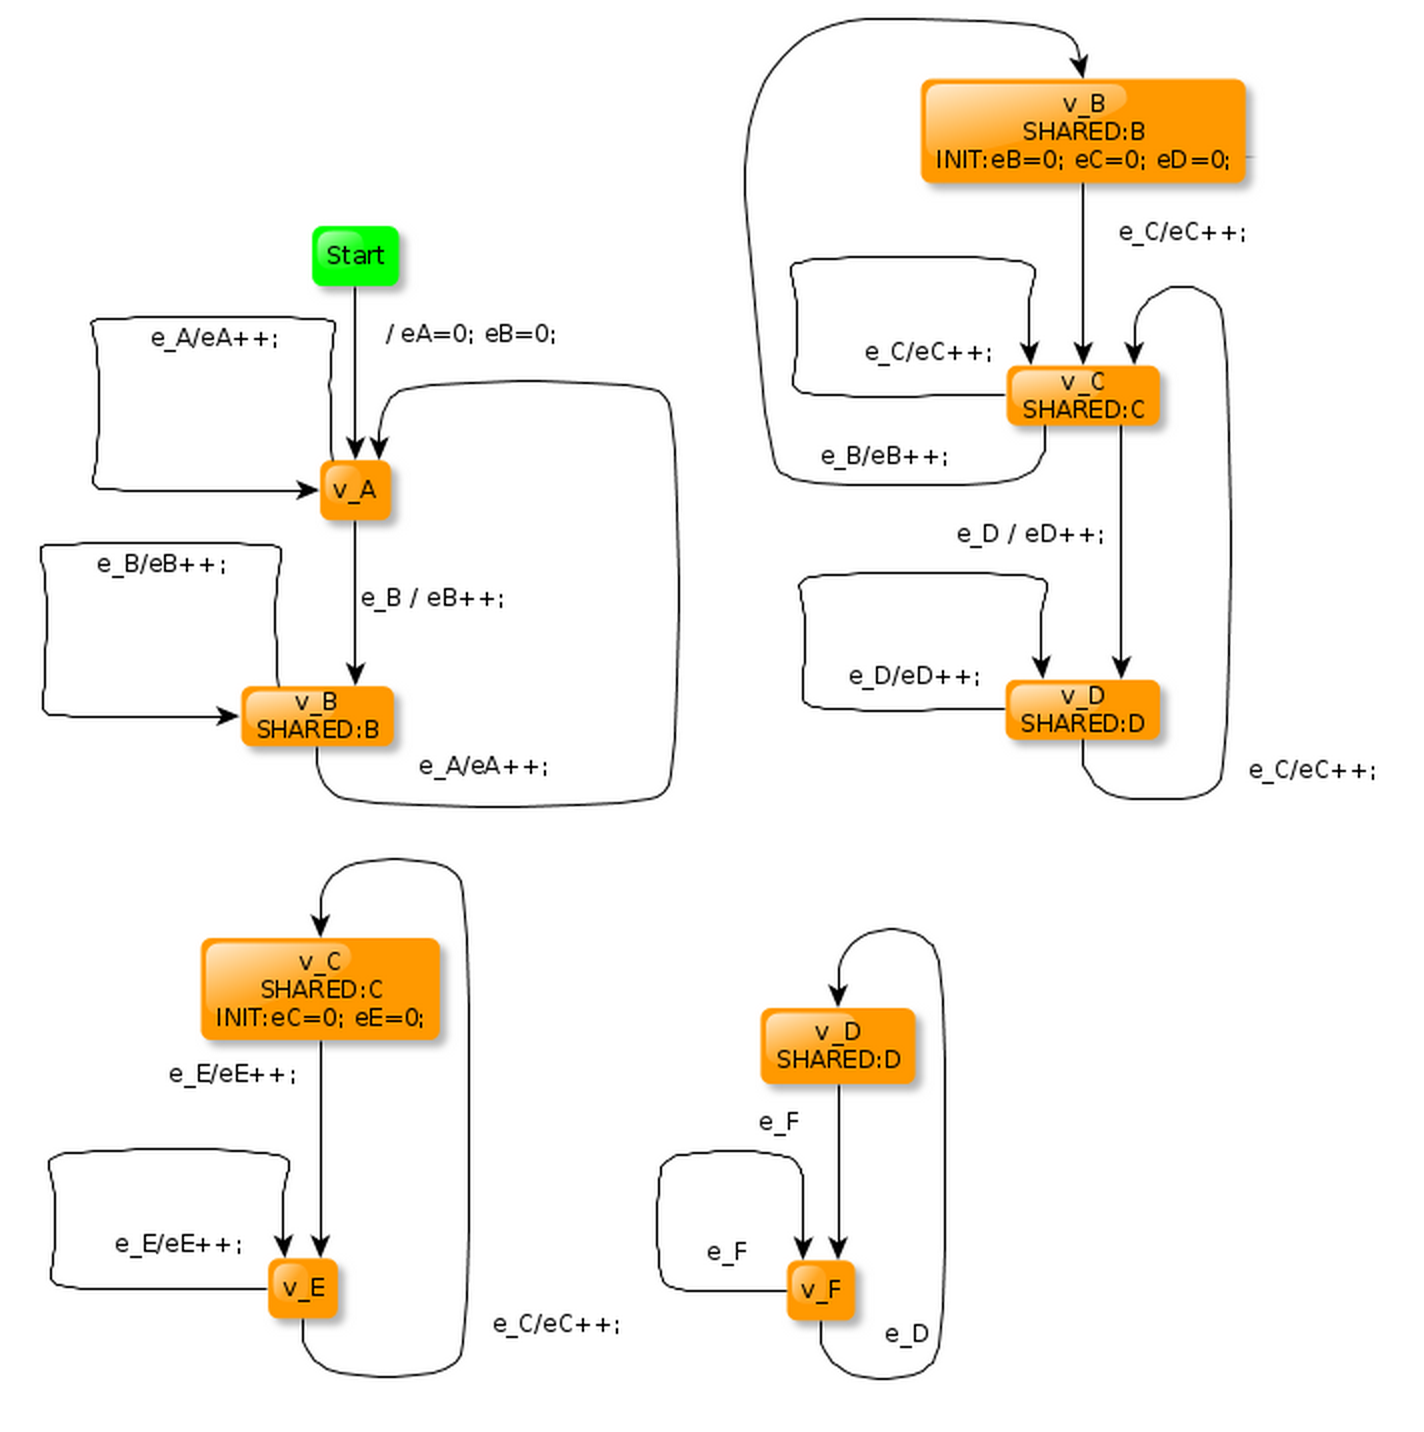
\includegraphics[width=0.9\textwidth]{figures/gw_multiple_models.png}
  \caption{Vier einzelne Modelle die in einer Traversierung durch SHARED-Knoten erreicht werden können.}
  \label{fig:gw_multiple_models}
\end{figure}

\todo[inline]{Formatierung paragraph - subparagraph}

\paragraph{Traversierung der Modelle} 
\label{sec:graphwalker_traversierung} 
Wie im ursprünglichsten Sinn des modellbasierten Tests gibt es in Graphwalker das Konzept der Testfälle nicht. Das \Gls{SUT} wird als gesamtes oder nur zu Teilen modelliert und das Testing wird durch die Auswahl eines Traversierungsalgorithmus angestoßen. Da die meisten Traversierungsalgorithmen von einer randomisierten Variante abhängen, wird das \Gls{SUT} bei jedem Testdurchlauf leicht unterschiedlich traversiert und damit getestet.\\
Durch die Modellierung des Modells, der Auswahl, sowie Einstellung eines Traversierungsalgorithmus, kann also bestimmt werden wie das \Gls{SUT} getestet werden soll. Dabei bietet Graphwalker bereits verschiedenste Algorithmen an, die sich für unterschiedliche Testzwecke eignen. Die meisten dieser Algorithmen basieren auf bekannten Graphalgorithmen und bieten durch die quelloffene Entwicklung volle Transparenz gegenüber dem Tester.

\subparagraph{Schnelle Traversierung - Smoke Tests}
Vor allem während der Testfallentwicklung und um kurze Testläufe zu realisieren eignet sich der A*-Algorithmus von Graphwalker. Er basiert auf dem bekannten A*-Suchalgorithmus von \citeauthor{hart_formal_1968} \cite{hart_formal_1968}. Dabei wird ein zu findender Knoten angegeben. Meist ist dies ein Knoten, der das Ende eines Workflows darstellt (im Quellcodebeispiel \ref{lst:runSmokeTest} ist dies der Knoten \texttt{v\_Browse}). Graphwalker durchschreitet das Testsystem in einem möglichst kurzen Pfad, wobei die zugrundeliegende Suchheuristik bei jedem Schritt angepasst wird.

\begin{lstlisting}[caption={Initialisierung eines Graphwalker Tests basierend auf dem A*-Suchalgorithmus.}, label=lst:runSmokeTest]
@Test
public void runSmokeTest() {
  new TestBuilder()
    .setPathGenerator(new AStarPath(new ReachedVertex("v_Browse")))
    .execute();
}
\end{lstlisting}

\subparagraph{Traversierung basierend auf Pfadabdeckung - Funktionaler Test}
Umfangreiche funktionale Tests einer komplexen Applikation, wie sie beispielsweise über Nacht gemacht werden, können mit Graphwalker unter anderem durch eine Zufallstraversierung mittels Angabe der gewünschten Pfadabdeckung realisiert werden. Falls eine einhundertprozentige Abdeckung eingestellt wird (wie im Codebeispiel \ref{lst:runFunctionalTest}), wird das Modell vom Startknoten (falls angegeben) aus traversiert, bis jede begehbare Kante traversiert wurde. Gegegebenenfalls werden weitere Durchläufe gestartet, falls es Teilgraphen gibt, die vom designierten Startknoten nicht erreichbar sind. 

\begin{lstlisting}[caption={Eine randomisierte aber vollständige Traversierung des Modells in Graphwalker.}, label=lst:runFunctionalTest]
@Test
public void runFunctionalTest() {
  new TestBuilder()
    .setPathGenerator(new RandomPath(new EdgeCoverage(100)))
    .execute();
    
}
\end{lstlisting}


\subparagraph{Traversierung mit Zeitangabe - Last- und Performance-Test}
Mit einer Traversierung der Modelle mit Zeitangabe (im Codebeispiel \ref{lst:runFunctionalTestTime} sind es 30 Sekunden) kann Graphwalker für Last- und Performance-Tests benutzt werden. Durch die Leichtgewichtigkeit von Graphwalker können Traversierungen auch parallel gestartet werden, um damit nicht unerhebliche Last auf ein Softwaresystem zu bringen. Um eine Traversierung mit Zeitangabe zu starten, wird ein Traversierungsalgorithmus (zum Beispiel mittels der Klasse \texttt{RandomPath}) und ein Zeitlimit angegeben.\\
Graphwalker bietet allerdings keine Möglichkeit, Metriken während des Durchlaufs zu erfassen. Diese Funktionalität muss durch andere Bibliotheken realisiert werden, was aber sehr einfach möglich ist.

\begin{lstlisting}[caption={Ein Graphwalker-Test wird angestoßen, der das Modell 30 Sekunden lang zufällig traversiert.}, label=lst:runFunctionalTestTime]
@Test
public void runFunctionalTest() {  
  new TestBuilder()
    .setPathGenerator(new RandomPath(new TimeDuration(30, TimeUnit.SECONDS)))
    .execute();
}
\end{lstlisting}


\subsection{Einbindung von anderen Technologien in Graphwalker Tests}
Graphwalker bietet mit dem Parsen des Modells, der Generierung der Java-Interfaces und der Traversierung des Modells nur das Grundgerüst für modellbasiertes Testen. Weil Graphwalkers volle Funktionalität in Java-Code gesteuert wird, sind keine von Herstellerseite wartungspflichtigen Schnittstellen zu anderen Systemen nötig. Das bedeutet, dass Werkzeuge zur Ansteuerung des \Gls{SUT} (Adapter-Code) problemlos verwendet werden können, sofern sie sich über reinen Java-Code ansteuern lassen. Dieser Umstand macht die Verwendung von Graphwalker extrem flexibel und gleichzeitig zukunftssicher, da auch ein Umstieg auf andere Technologien problemlos möglich ist.\\
Üblicherweise befindet sich in den Knoten (diese stellen einen Zustand dar) Code, der auf das \Gls{SUT} überprüfend zugreift (\textit{Assertions}). In den Kanten (stellen eine Aktion dar) befindet sich Code, der eine Eingabe am \Gls{SUT} macht.\\
Auf Schnittstellenebene kann beispielsweise SoapUI als Verbindungsstück zum \Gls{SUT} gewählt werden. Die Methode im Beispiel \ref{lst:graph_soap} implementiert das von Graphwalker aus dem Modell erzeugte Interface \texttt{e\_InvalidCredentials}. Die Methode repräsentiert eine Kante (erkennbar am Präfix \texttt{e}), die Login-Eingaben macht, die vom \Gls{SUT} als ungültig erkannt werden sollten. In der Methode wird eine Referenz zur SoapUI-Schnittstelle hergestellt. Das dazugehörige SoapUI-Projekt liegt vorbereitet an einem definierten Pfad. Im Code wird außerdem der auszuführende Testfall definiert (hier \texttt{ValidLogin}). Zuletzt wird der SoapUI-Testfall angestoßen und der Fehlerbericht gegebenenfalls abgefangen.

\begin{lstlisting}[caption={Eine Methode, die ein von Graphwalker erzeugtes Interface implementiert und einen SoapUI-Testfall anstößt.}, label=lst:graph_soap]
@Override
public void e_ValidCredentials() {

    //Invoke SoapUI testcase with valid credentials
    SoapUITestCaseRunner runner = new SoapUITestCaseRunner();
    runner.setProjectFile(SOAPUI_PROJECT_PATH);
    runner.setTestSuite("ValidLogin");
    try {
        runner.run();
    } catch (Exception e) {
        report.addTestCaseWithError(ErrorType.EDGE_ERROR.toString(), System.currentTimeMillis(), "Error while validating credentials", e.getStackTrace().toString());
    }
}
\end{lstlisting}

An dieser Stelle kann also eine Vielzahl von Aufrufen passieren:

\begin{itemize}
\item \textbf{Adapter-Code:} Wie im Codebeispiel \ref{lst:graph_soap} kann ein fremdes Framework angesprochen werden, um auf das \Gls{SUT} zuzugreifen. In der Fallstudie (siehe Abschnitt \ref{sec:fallstudie}) wurde dabei hauptsächlich SoapUI und RESTassured\footnote{RESTassured Testing Library \url{https://github.com/jayway/rest-assured}} verwendet. Aber auch große kommerzielle Testwerkzeuge bieten Java-Schnittstellen an, die an diesen Stellen angesprochen werden können.
\item \textbf{Reporting und Historisierung:} Genauso können an dieser Stelle Aufrufe zu externen Systemen erfolgen, die von den verschiedensten Parteien verwendet werden, um den Qualitätsstatus des \Gls{SUT} zu verwalten (sogenannte \textit{Application Lifecycle} Tools). 
\item \textbf{Testdatenmanagement:} Auch möglich und oftmals sinnvoll ist der Zugriff auf eine Komponente oder ein externes System welches für das Testdatemanagement zuständig ist. Das kann ein Datenbankzugriff sein oder auch eine Anfrage an ein über das Netzwerk oder Internet angeschlossenes Testdatenwerkzeug.
\end{itemize}


